\documentclass[12pt]{article}

\usepackage[utf8]{inputenc}
\usepackage[T1]{fontenc}
\usepackage{microtype}
\usepackage[brazil]{babel}
\usepackage{csquotes}
\usepackage[sortcites=true, backend=biber]{biblatex} 
\usepackage{bm}
\usepackage{times}
\usepackage{amsfonts}
\usepackage{amsmath}
\usepackage{amsthm}
\usepackage{graphicx}
\usepackage{indentfirst}
\usepackage{float}
\usepackage{hyperref}
\usepackage{booktabs} % Para tabelas profissionais
\usepackage{caption}
\usepackage{algorithm}
\usepackage{algpseudocode}

\newtheorem{observation}{Observação}
\newtheorem{definition}{Definição}
\newtheorem{proposition}{Proposição}
\newtheorem{example}{Exemplo}
\DeclareMathOperator{\prox}{prox}
\DeclareMathOperator*{\argmin}{arg\ min}
\newcommand{\norm}[1]{\left\lVert#1\right\rVert}

\addbibresource{bibliography.bib}

\title{Influência do Uso de Busca Linear Exata na Convergência de Métodos Acelerados de Gradiente Proximal}
\author{Orientador: Elias Salomão Helou Neto\\Aluno: Gabriel Ligabô Baba}


\begin{document}
\begin{titlepage}
	\begin{center}
		{\large \sc UNIVERSIDADE DE SÃO PAULO} \\
		{\large \sc INSTITUTO DE CIÊNCIAS MATEMÁTICAS E DE COMPUTAÇÃO}\\[0.7cm]
		{\small \sc DEPARTAMENTO DE MATEMÁTICA APLICADA E ESTATÍSTICA}
		
		\vspace{4cm}
		
		{\large \sc Relatório Científico Semestral}\\
		\rule{\linewidth}{2pt}
		
		\vspace{0.7em}
		{\Large \bfseries Influência do Uso de Busca Linear Exata na Convergência de Métodos Acelerados de Gradiente Proximal}
		\vspace{0.2em}
		
		\rule{\linewidth}{2pt} \\
		{\small \sc Linha de Fomento: Bolsa no País - Regular - Iniciação Científica}
	\end{center}
	
	
	\vspace{1.8cm}
	
	\begin{flushleft}
		\textbf{Processo FAPESP}: 2025/12023-2\\
		\textbf{Período de vigência}: 01/09/2025 a 31/08/2026\\
	\end{flushleft}
	
	\vspace{1.8cm}
	
	\begin{minipage}{0.43\textwidth}
		\emph{Bolsista:}\\
		Gabriel Ligabô Baba
	\end{minipage}
	\hspace{1cm}
	\begin{minipage}{0.43\textwidth}
		\emph{Orientador:}\\
        Elias Salomão Helou Neto	
	\end{minipage}
	
	\vfill
	
	\begin{center}
		\makeatletter
		São Carlos -- SP \\
		\@date
		\makeatother
	\end{center}
\end{titlepage}

\newpage
\tableofcontents
\newpage

\section{Introdução}
Métodos de otimização são peça-chave em reconstrução de imagens médicas, especialmente em tomografia computadorizada. Os dados adquiridos por esta técnica consistem em uma amostragem ruidosa da transformada de Radon, o que leva à necessidade da adição de termos de regularização ao modelo de otimização, para que assim o ruído contido nos dados não seja excessivamente amplificado na imagem reconstruída. Muitas das possíveis escolhas para o termo regularizador não são suaves, mas são convexas e prox-amigáveis, levando ao uso de algoritmos de otimização do tipo gradiente proximal acelerado. Este projeto aborda um ponto específico e pouco explorado: propomos substituir as estratégias de tamanho de passo usuais (e.g., passo fixo ou determinado por busca inexata com critério de descida suficiente) no algoritmo FISTA (Fast Iterative Shrinkage-Thresholding Algorithm). Em seu lugar, investigar-se-á o uso de uma busca linear exata para determinar o tamanho de passo. Especificamente, usaremos um termo de quadrados mínimos na parcela de consistência e calcularemos analiticamente o passo que minimiza tal parcela ao longo da direção de máxima descida. A meta é medir, de forma objetiva, como tal escolha afeta a convergência em iterações e o tempo de computação, além da qualidade de reconstrução em dados de tomografia computadorizada.

\section{Fundamentação Matemática}

\begin{definition}
Um subconjunto $X \subset \mathbb{R}^n$ é dito convexo se, para todo $x, y \in X$ e $\lambda \in [0,1]$, ele satisfaz que:

\[
\lambda x + ( 1 - \lambda ) y
\] também pertence a X.
\end{definition}

\begin{definition}
Seja $X \subset \mathbb{R}^n$. Seja $f : X \to \mathbb{R}$, $f$ é dita convexa se, para quaisquer $x,y \in X$ e $\lambda \in [0,1]$ temos:

\[
f(\lambda x + ( 1-\lambda ) y ) \leq \lambda f(x) + ( 1 - \lambda )f(y)
\]
\end{definition}

As funções convexas nos dão algumas propriedades fundamentais, como as seguintes:

\begin{proposition}
Seja $f$ uma função de classe $C^1$. Então $f$ é convexa em $X$, se e somente se, para todo $x,y \in X$
\[
f(y) \geq f(x) + \nabla f(x)^T(y-x)
\]
\end{proposition}
Em outras palavras, isso significa que a aproximação de primeira ordem de Taylor sempre subestima o valor real da função.

\begin{proposition}
    
Seja $f$ uma função de classe $C^2$. Seja $X \subset \mathbb{R}^n$, então $f$ é convexa se e somente se, para todo $x \in X$:
\[
\nabla^2 f(x) \geq 0
\]
\end{proposition}

\begin{definition}

Dizemos que um vetor $g \in \mathbb{R}^n$, onde $X$ é convexo, é um subgradiente de $f : X \to \mathbb{R}$ convexa em um ponto $x \in X$ se, para todo $y \in X$ a seguinte desigualdade for satisfeita:

\[
f(y) \geq f(x) + g^T (y-x)
\]
\end{definition}

Em outras palavras, $g$ define um hiperplano de suporte para o epígrafo de $f$ no ponto $(x, f(x))$. Se $f$ for diferenciável, então o subgradiente é o próprio gradiente da função.
\begin{observation}
    O epígrafo de uma função é definido como $epi(f) = \{(x,y) : x \in \mathbb{R}^n, y \in \mathbb{R}, f(x) \leq y\}$
\end{observation}

\begin{definition}
O conjunto de todos os subgradientes em um ponto $x \in X$ é chamado de subdiferencial de $f$ em $x$. A notação usada é:

\[
\partial f(x) = \{ g \in \mathbb{R}^n : g^T(y-x) \leq f(y) - f(x), \forall y \in X\}
\]
\end{definition}

% \begin{example}
% Considere $f(x) = |x|$. 

% Para $x < 0$ o subgradiente é único, ou seja, é a própria derivada, então $\partial f(x) = \{-1\}$. 

% Para $x>0$ o subgradiente também é único, ou seja, é igual ao gradiente. Nesse caso $\partial f(x) = \{1\}$

% Quando $x=0$, essa função não é diferenciavel, no entanto, qualquer $g \in [-1,1]$ satisfaz a desigualdade $f(y) \geq f(x) + g^T(y-x)$. Sendo assim,
% $\partial f(0) = [-1,1]$.
% \end{example}

\begin{definition}
Seja $f : X \to \mathbb{R}$ uma função convexa. Definimos o operador proximal como sendo:

\[
\prox_f(v) = \argmin_{x\in X}\{f(x) + \frac{1}{2}\norm{x - v}_2^2 \} 
\]
\end{definition}
A função $f$ também pode ser multiplicada por uma constante $\lambda > 0$. Então o operador proximal fica:

\[
\prox_{\lambda f}(v) = \argmin_{x\in X}\{f(x) + \frac{1}{2\lambda}\norm{x - v}_2^2 \} 
\]

\begin{definition}
Uma função f é dita $L_f$-suave se seu gradiente é Lipschitz contínuo com parâmetro $L_f$. Isto é:
    \[
    \norm{\nabla f(x) - \nabla f(y)}_2 \leq L_f \norm{x - y}_2
    \]
\end{definition}

\begin{proposition}
No problema de mínimos quadrados definido por $f(x) = \frac{1}{2} \norm{Ax - b}_2^2$, o tamanho de passo que miniza a função ao longo da direção $d_k$ é dado por:
\[
\lambda_k = -\frac{\nabla f(x_k)^T d_k}{d_k^T Qd_k}
\]
\end{proposition}, onde $Q = A^TA$

\subsection{ISTA e FISTA}
\label{problema}
Quando estamos lidando com o problema compósito:

\[
\min F(x) = f(x) + \gamma g(x)
\]
onde:
 
$f(x)$ é uma função suave e convexa


$g(x)$ é uma função convexa não suave.

Uma possível forma de resolvê-lo é utilizando um método chamado de ISTA (\textit{Iterative Shrinkage-Thresholding Algorithm}). A ideia por trás deste método, é aproveitar da suavidade de $f$ para realizar um passo da descida do gradiente e, em seguida, corrigir o efeito da parte não diferenciável via operador proximal. Então fazemos:

\begin{algorithm}[H]
\caption{ISTA}
\begin{algorithmic}[1]
\State \textbf{Entrada:} $x_0 \in \mathbb{R}^n$, passo $\lambda > 0$.
\For{$k = 0, 1, 2, \dots$}
    \State $x_{k+1} = \operatorname{prox}_{\gamma \lambda g} ( x_k - \lambda \nabla f( x_k ) )$
\EndFor
\State \textbf{Retorno:} Solução aproximada $x^*$.
\end{algorithmic}
\end{algorithm}

Uma variação mais eficiente é o FISTA (\textit{Fast Iterative Shrinkage-Thresholding Algorithm}) \cite{doi:10.1137/080716542}, que utiliza o momento de Nesterov para acelerar a convergência.

\begin{algorithm}[H]
\caption{FISTA}
\begin{algorithmic}[1]
\State \textbf{Entrada:} $x_0 \in \mathbb{R}^n$, $\lambda > 0$.
\State \textbf{Inicialização:} $y_1 = x_0$, $t_1 = 1$.
\For{$k = 1, 2, \dots$}
    \State $x_k = \operatorname{prox}_{\gamma \lambda g} ( y_k - \lambda \nabla f( y_k ) )$
    \State $t_{k+1} = \frac{1 + \sqrt{ 1 + 4 t_k^2 }}{2}$
    \State $y_{k+1} = x_k + \left( \frac{t_k - 1}{t_{k+1}} \right) ( x_k - x_{k-1} )$
\EndFor
\State \textbf{Retorno:} Solução aproximada $x^*$.
\end{algorithmic}
\end{algorithm}


Um dos casos que será foco deste trabalho, é a utilização de $g(x) = \norm{Hx}_1$, onde $H$ é uma transformada \textit{wavelet} ortonormal auto-adjunta. Neste caso, o operador proximal é facilmente computável, tendo fórmula fechada dada por:

\[
\prox_{\lambda \gamma g}(x) = H^T \mathcal{S}_{\lambda \gamma}(Hx)
\]
onde $\mathcal{S}_{\lambda \gamma}$ é o operador de \textit{soft-thresholding}.

Um outro caso de interesse é quando $g(x) = TV(x)$, onde $x \in \mathbb{R}^{m \times n}$:

\[
TV(x) = \sum_{i=1}^{m-1} \sum_{j=1}^{n-1} \sqrt{(x_{i,j} - x_{i+1,j})^2 + (x_{i,j} - x_{i,j+1})^2} + \sum_{i=1}^{m-1} |x_{i,n} - x_{i+1,n}| + \sum_{j=1}^{n-1} |x_{m,j} - x_{m,j+1}|
\]

Neste caso, não existe forma fechada para o cálculo do operador proximal, mas o algoritmo rápido apresentado em \cite{5173518} será implementado na linguagem python. 
\section{Resultados}

\subsection{Métodos sem Regularização para \textit{Deblurring} de Imagens}

Nessa etapa do projeto, comparamos diversos métodos: máxima descida com passo fixo (MDPF), máxima descida com busca linear exata (MDBE), método de Nesterov com passo fixo, método de Nesterov com critério de descida suficiente (com \textit{backtracking}), método de Nesterov com busca linear exata e gradientes conjugados para reconstrução de imagens borradas. O objetivo é:

\begin{equation*}
\min_x \|Ax - b\|_2^2
\end{equation*}
onde $A$ representa um operador de convolução (responsável pelo \textit{blur}), $x$ a imagem original a ser recuperada e $b$ a imagem borrada.

Esses métodos foram comparados em termos de iterações e tempo de convergência visando analisar a influência do uso da busca linear exata.
Implementamos todos os métodos  em linguagem de programação Python com o uso de bibliotecas como Scipy, Numpy e Matplotlib. A imagem a ser recuperada foi a \textit{coffee} da biblioteca \textit{scikit-image}.

Inicialmente, foi utilizado um \textit{grid search} para encontrar o melhor parâmetro de tamanho de passo, conforme apresentado na Figura \ref{fig:tamanho_passo_sreg}:

\begin{figure}[H]
    \centering
    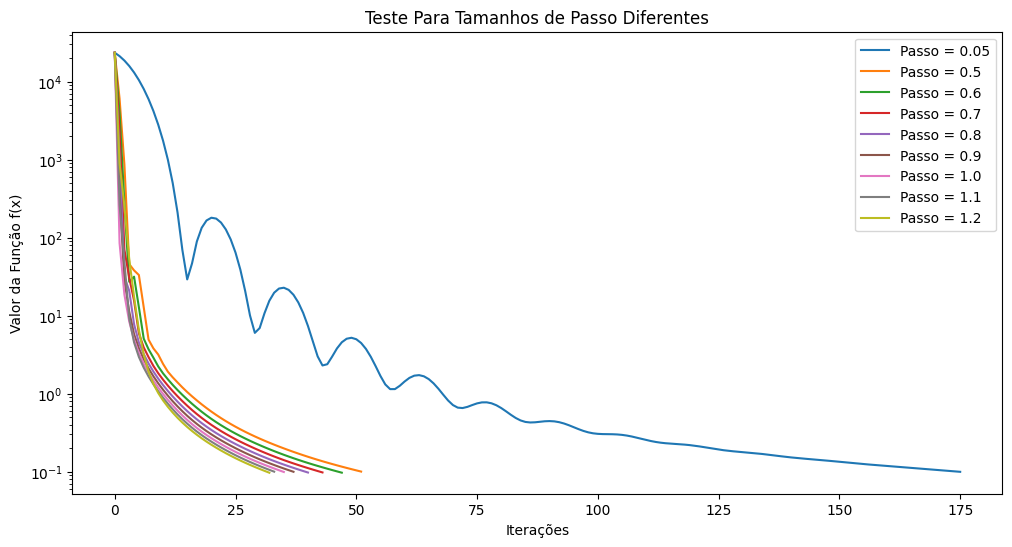
\includegraphics[width = 0.9\textwidth]{tamanho_passo_semreg.png}
    \caption{Análise de tamanho de passo.}
    \label{fig:tamanho_passo_sreg}
\end{figure}

Além disso, nesse cenário de experimento controlado, foi possível estimar a constante de Lipschitz ($L = 0.9996$). Sendo assim, decidiu-se por utilizar o melhor tamanho de passo fixo ($\lambda = \frac{1}{L}$) que é de aproximadamente $\lambda = 1$.

Em todos os experimentos desse tipo de problema, utilizou-se a avaliação do valor da função objetivo $f$ como critério de parada. Como operador de convolução $A$, foi adotado um kernel de média de dimensões $7 \times 7$. Em um experimento inicial, utilizou-se um limite máximo de 1000 iterações como critério de parada e uma tolerância de $1.0 \times 10^{-2}$.
Os resultados obtidos em termos de número de iterações, tempo para convergência e qualidade da reconstrução (PSNR) podem ser observados na Tabela \ref{tab:resultados} e nas Figuras \ref{fig:conv_iter_sreg} e \ref{fig:conv_tempo_sreg}.

\begin{table}[H]
    \centering
    \caption{Convergência dos Métodos}
    \label{tab:resultados}
    \begin{tabular}{lccc}
        \toprule
        \textbf{Método} & \textbf{Iterações} & \textbf{Tempo (segundos)} & \textbf{PSNR (dB)} \\
        \midrule
        Máxima Descida Passo Fixo & 1000 & 41.64 & 30.4\\
        Máxima Descida Busca Exata & 849 & 58.73 & 31.23\\
        Nesterov Passo Fixo & 109 & 4.8 & 31.25\\
        Nesterov Busca Exata & 94 & 6.51 & 31.25\\
        Nesterov Backtracking  & 99 & 6.85 & 31.24\\
        Gradientes Conjugados & 59 & 4.85 & 31.37\\
        \bottomrule
    \end{tabular}

    \vspace{0.2cm}
    {\footnotesize Menores valores de iterações e tempo indicam melhor desempenho computacional.}
\end{table}

\begin{observation}
    A métrica PSNR (Peak Signal-to-Noise Ratio) é amplamente utilizada para avaliar a qualidade de reconstrução de imagens, sendo que valores mais elevados indicam menor distorção em relação a imagem de referência.
\end{observation}


\begin{figure}[H]
    \centering
    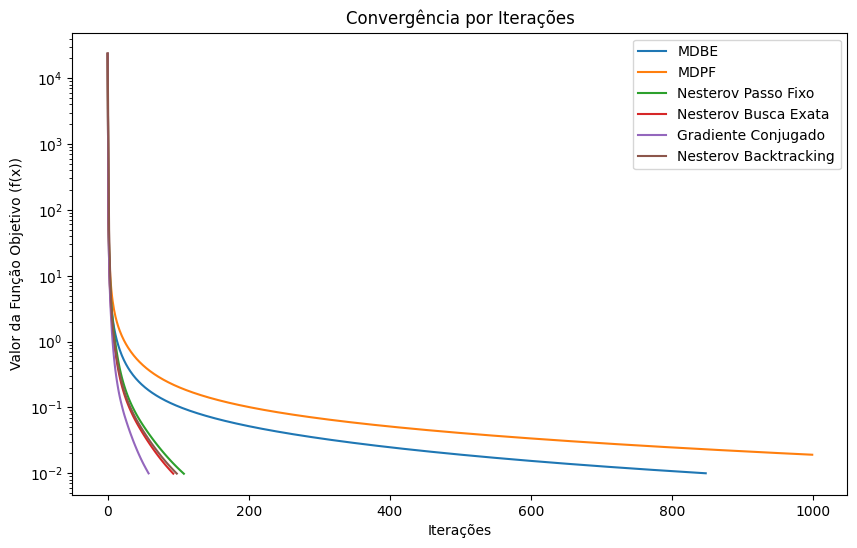
\includegraphics[width = 0.9\textwidth]{conv_iter_sreg.png}
    \caption{Gráfico de convergência pelo número de iterações}
    \label{fig:conv_iter_sreg}
    \vspace{0.2cm}
{\footnotesize Curvas mais baixas e que atingem valores reduzidos em menos iterações indicam melhor desempenho do método.}
\end{figure}

\begin{figure}[H]
    \centering
    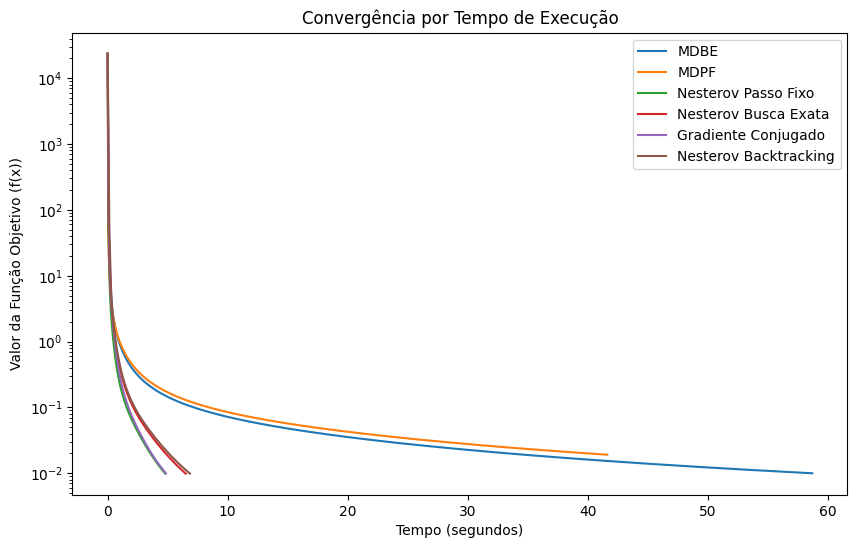
\includegraphics[width = 0.9\textwidth]{conv_tempo_sreg.png}
    \caption{Gráfico de convergência pelo tempo de execução}
    \label{fig:conv_tempo_sreg}
    \vspace{0.2cm}
{\footnotesize Curvas mais baixas e que atingem valores reduzidos em menor tempo indicam melhor desempenho do método.}

\end{figure}

\begin{observation}
    É importante citar que o tamanho de passo $\lambda = 1.2$ foi o utilizado na implementação do Nesterov com \textit{backtracking}. Além disso, veja que é improvável que esse método apresente desempenho superior do que o passo fixo na nossa situação de simulação, já que estamos utilizando o tamanho de passo ótimo $\lambda = \frac{1}{L}$ para o Nesterov com passo fixo.
\end{observation}

Esse primeiro experimento evidencia que em termos de iterações, a ordem dos métodos mais eficientes é: gradientes conjugados, Nesterov com busca linear exata, Nesterov com \textit{backtracking}, Nesterov com passo fixo e máxima descida com busca exata. O método de máxima descida com passo fixo atingiu o limite máximo de iterações sem satisfazer o critério de convergência. Embora isso mostre que o uso da busca linear exata para definir o tamanho de passo reduza o número de iterações para atingir a convergência, ainda resta avaliar se o tempo computacional é reduzido. Quando se trata do método de Nesterov, as figuras nos apresentam que ao utilizar a busca exata, de fato há um ganho de performance tanto em números de iterações quanto na redução do tempo para convergir em relação ao método que utiliza \textit{backtracking}. Isso é importante pois, por mais que ambos percam para o Nesterov com passo fixo ao utilizar o tamanho de passo ótimo ($\lambda = \frac{1}{L}$), em aplicações reais é custoso computacionalmente estimar a constante de Lipschitz. No entanto, nesse caso onde a função objetivo é uma quadrática, há a possibilidade de utilizar o método dos gradientes conjugados, que nesses experimentos performou melhor que todos os outros algoritmos. Portanto, a ordem de eficiência por tempo computacional é dada por: Nesterov passo fixo, gradientes conjugados, Nesterov com busca exata, Nesterov com \textit{backtracking} e máxima descida com busca exata. Nesse teste o método de máxima descida com passo fixo atingiu o número de iterações máxima sem alcançar a tolerância desejada.
Quanto à qualidade da imagem recuperada, os valores de PSNR na Tabela \ref{tab:resultados} corroboram a superioridade dos métodos acelerados. Enquanto a Máxima Descida com passo fixo resultou no menor PSNR ($30.4$ dB) por não atingir a convergência plena, os métodos de Nesterov e Gradientes Conjugados estabilizaram em patamares superiores. 

Vale destacar que o método de Gradientes Conjugados, além da eficiência em iterações, apresentou o maior PSNR ($31.37$ dB), evidenciando que a eficiência computacional foi acompanhada de uma reconstrução mais fiel. Observa-se também que as diferentes estratégias para o método de Nesterov atingiram valores de PSNR praticamente idênticos (aproximadamente $31.25$ dB), o que indica que, embora o tipo de busca linear altere a velocidade de convergência, o algoritmo consistentemente converge para a mesma vizinhança do ponto ótimo.
Outro experimento efetuado foi utilizando um limite de 200 iterações e uma tolerância de $1.0 \times 10^{-5}$. Com isso, chegamos nos resultados da Tabela \ref{tab:resultados_2}.


\begin{table}[H]
    \centering
    \caption{Comparação por Iteração}
    \label{tab:resultados_2}
    \begin{tabular}{lcc}
        \toprule
        \textbf{Método} & \textbf{Iterações} & \textbf{Tempo (segundos)} \\
        \midrule
        Máxima Descida Passo Fixo & 200 & 8.08\\
        Máxima Descida Busca Exata & 200 & 13.44 \\
        Nesterov Passo Fixo & 200 & 8.11\\
        Nesterov Busca Exata & 200 & 13.35 \\
        Nesterov Backtracking  & 200 & 13.63\\
        Gradientes Conjugados & 200 & 16.02\\
        \bottomrule
    \end{tabular}

\vspace{0.2cm}
{\footnotesize Aqui não necessariamente quanto menor o tempo melhor, temos que avaliar a qualidade da reconstrução}

\end{table}

Neste experimento, a análise prioriza a qualidade da reconstrução obtida por cada método, avaliada por meio da métrica PSNR, conforme ilustrado na Figura \ref{fig:qual_reconst_2}, que evidencia a superioridade do método dos gradientes conjugados.

\begin{figure}[H]
    \centering
    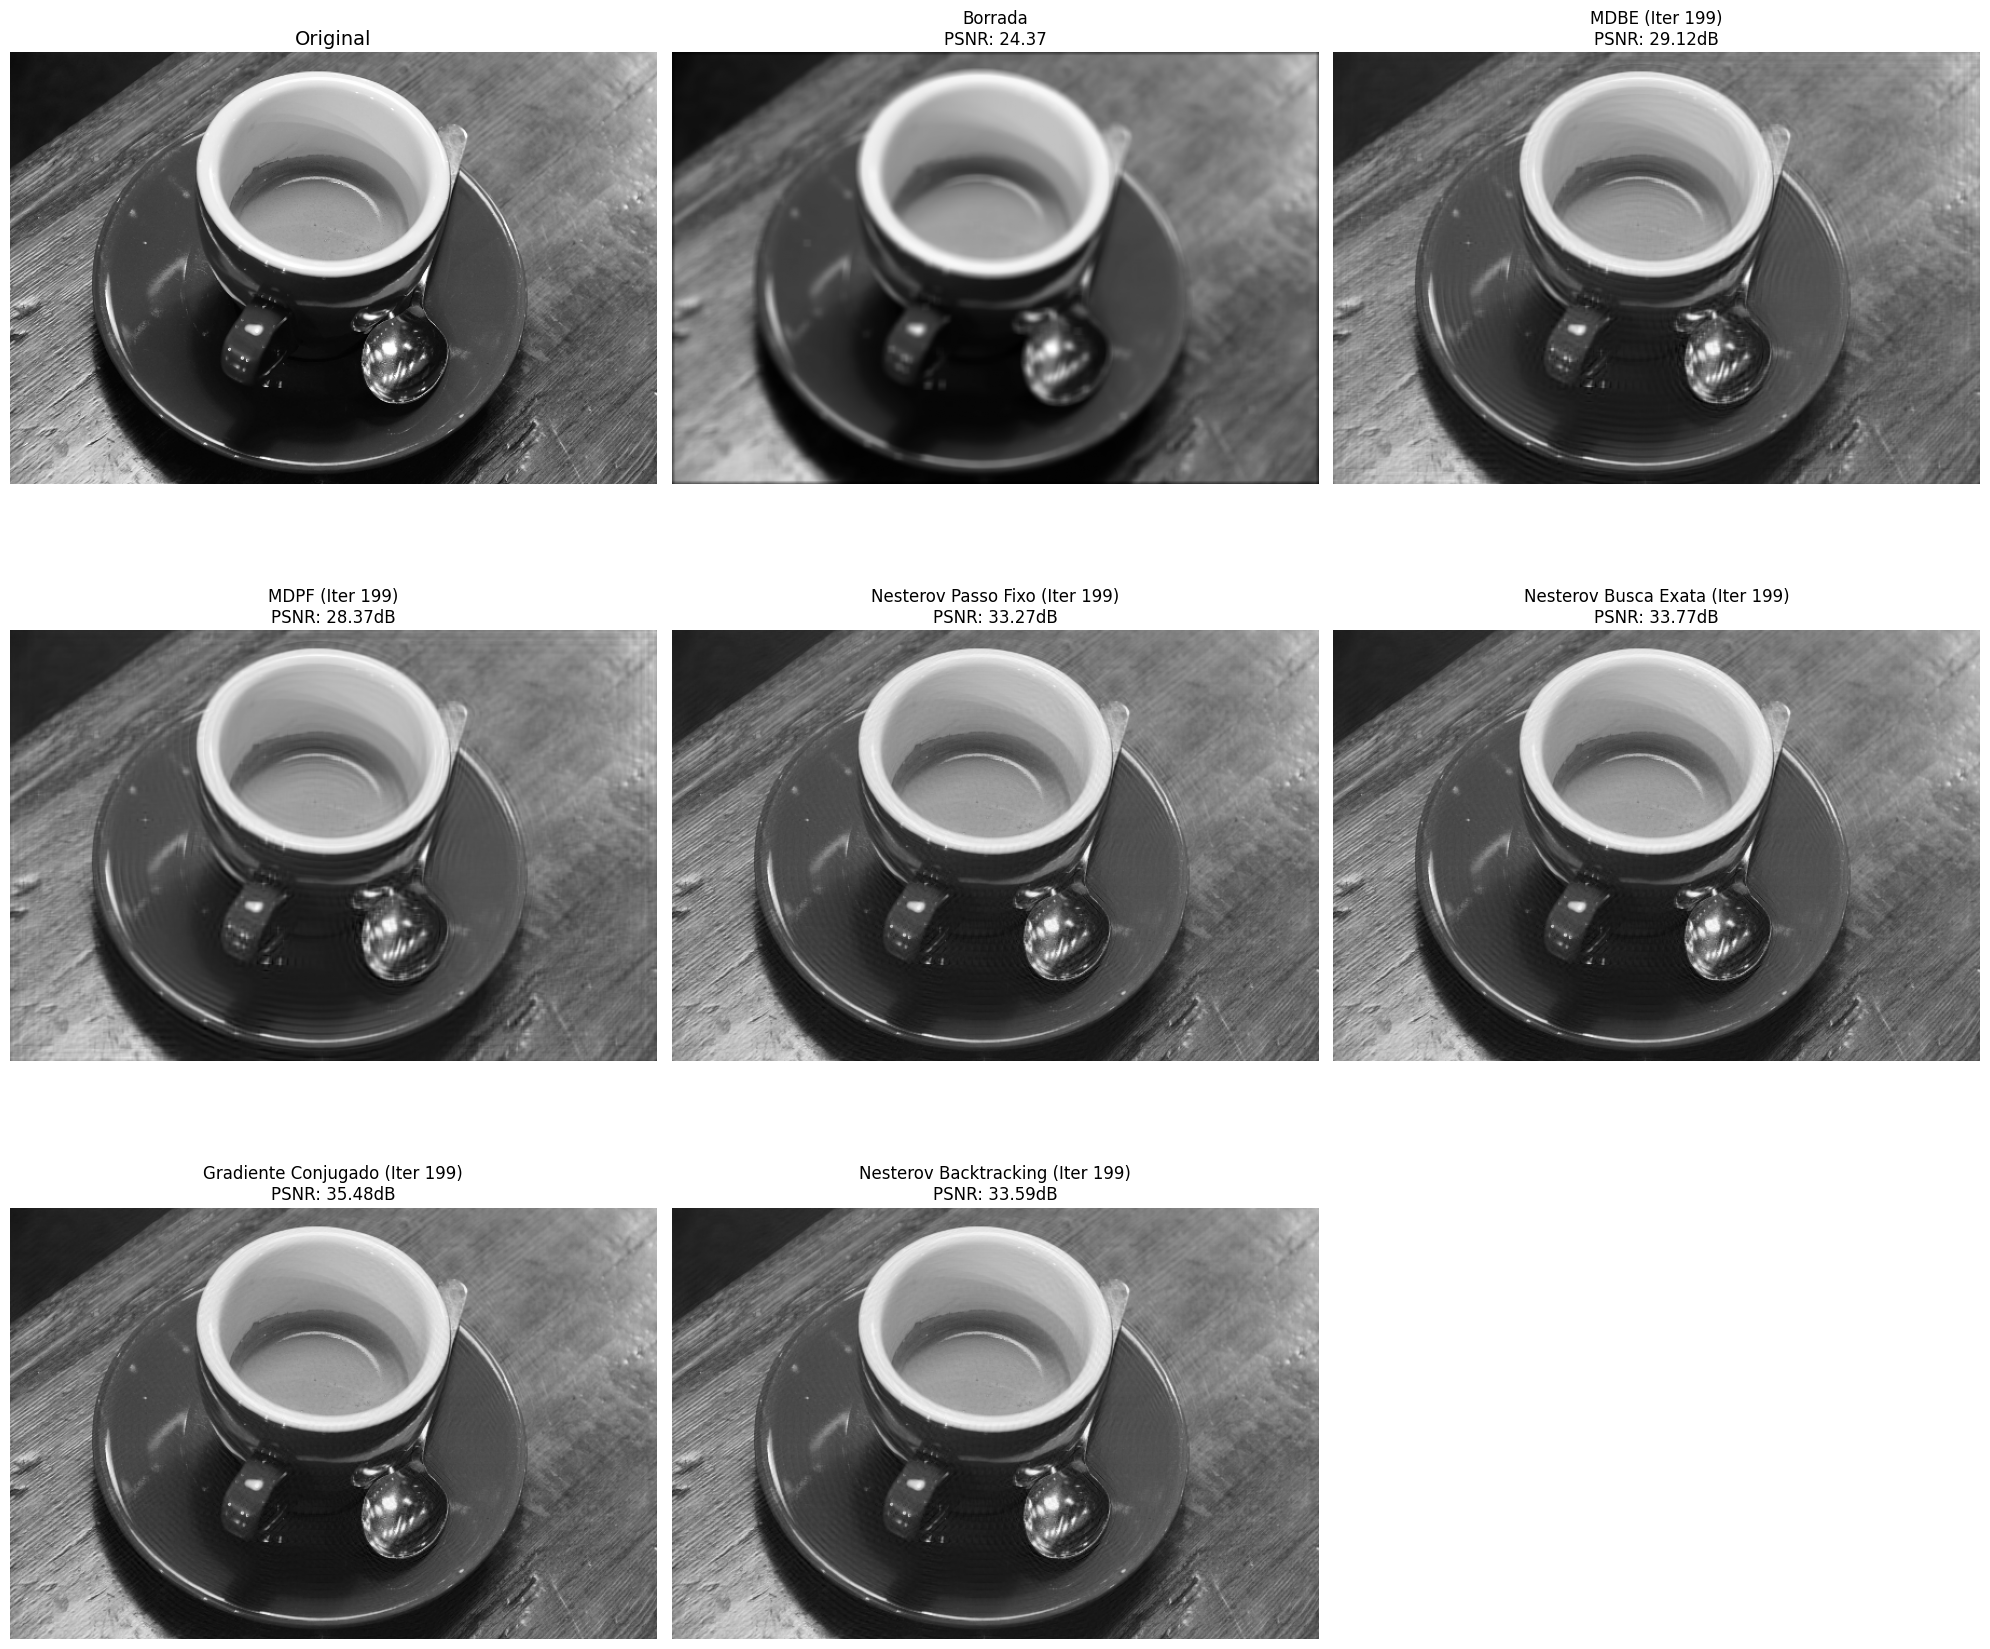
\includegraphics[width = 1\textwidth]{reconstrucao_200_iter.png}
    \caption{Qualidade da Reconstrução}
    \label{fig:qual_reconst_2}  
\end{figure}

Além desses experimentos, foram feitos alguns comparando o uso de busca exata com o backtracking no método de Nesterov. Rodando os métodos por 200 iterações, temos que o algoritmo que utiliza busca exata atinge o limite de iterações em 13.51 segundos, já utilizando \textit{backtracking} leva 13.58 segundos. Na reconstrução vista na Figura \ref{fig:qual_reconst_nesterov}, fica claro que o uso da busca exata traz vantagens tanto em tempo de convergência como na qualidade da imagem reconstruída em relação ao uso de \textit{backtracking}
\begin{figure}[H]
    \centering
    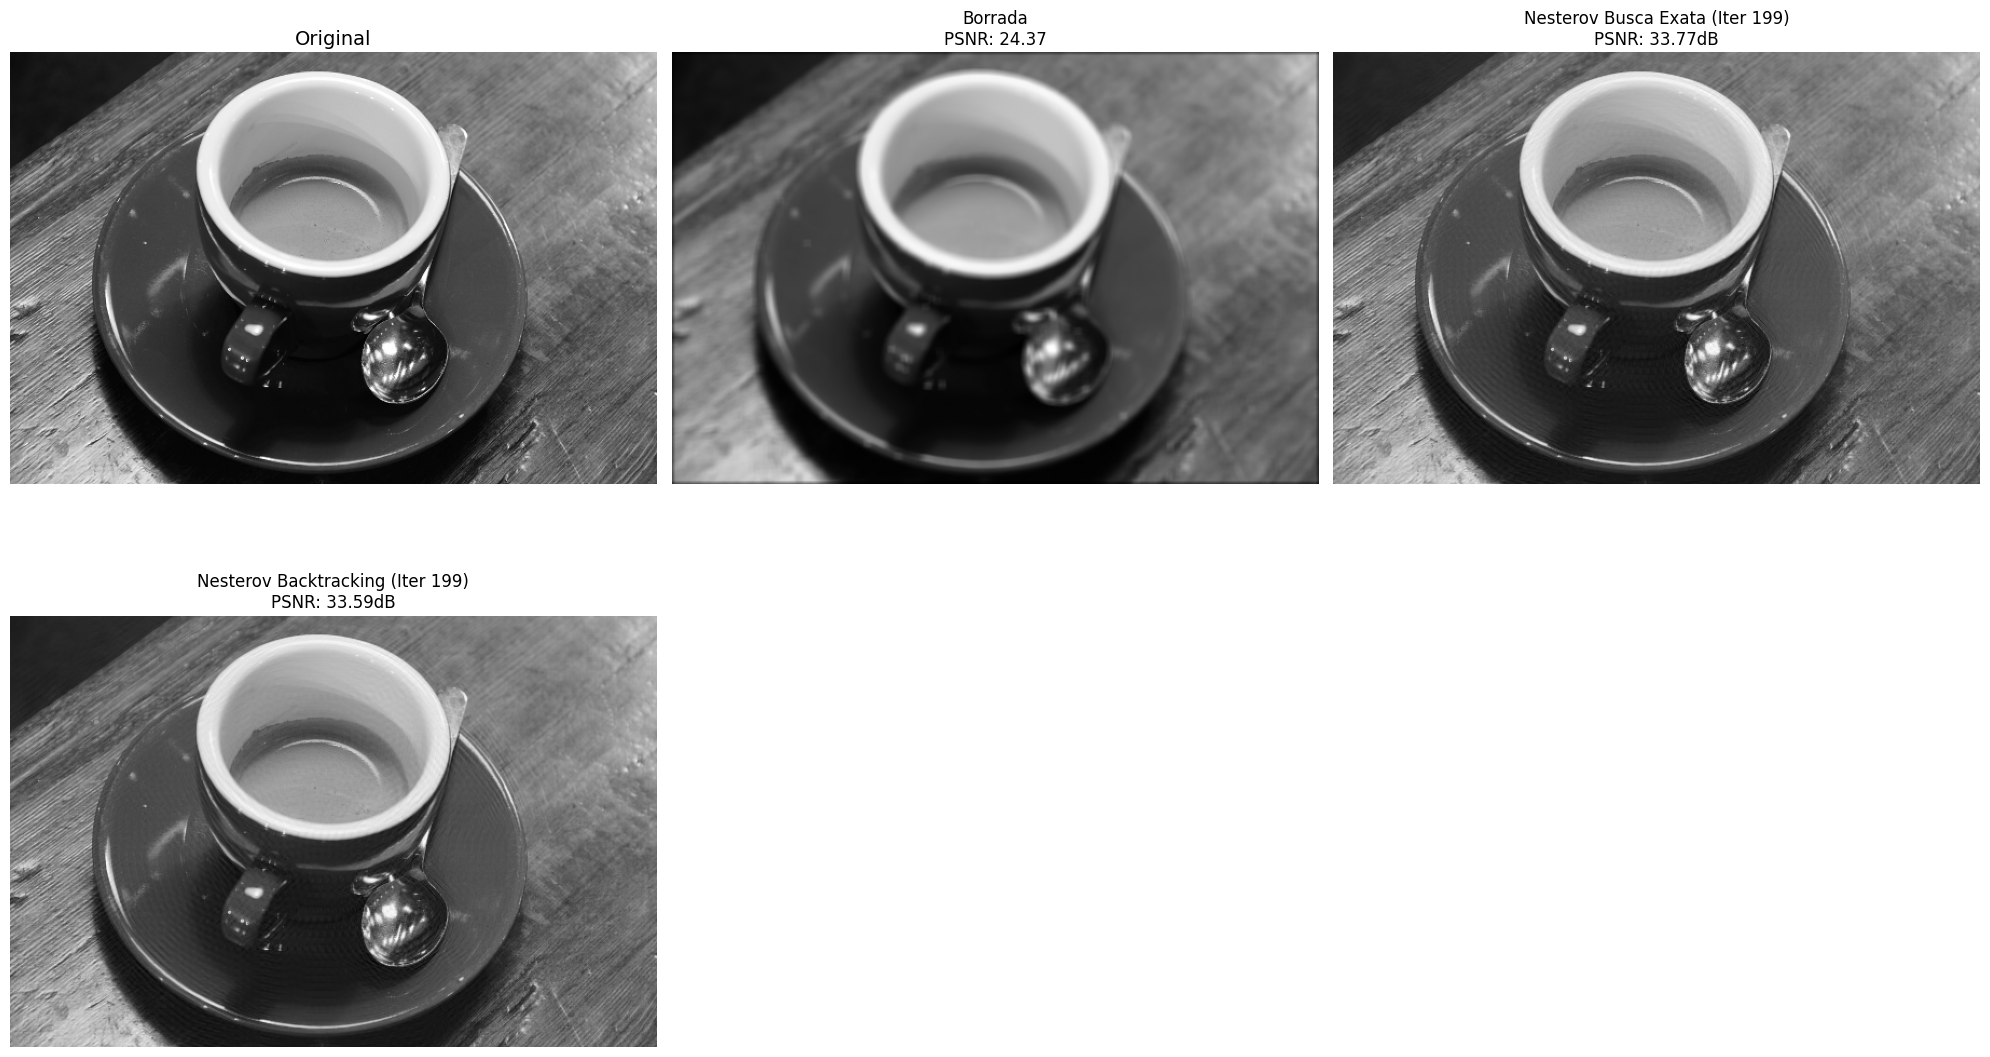
\includegraphics[width = 1\textwidth]{reconstrucao_nesterov.png}
    \caption{Qualidade da Reconstrução}
    \label{fig:qual_reconst_nesterov}
\end{figure}

Por último, comparou-se o método dos gradientes conjugados com o método de Nesterov utilizando busca linear exata. O experimento se deu considerando uma tolerância de $1.0 \times 10^{-5}$ e um limite máximo de 1500 iterações. Os resultados podem ser vistos na Tabela \ref{tab:resultados_3} em conjunto com a qualidade da reconstrução na Figura \ref{fig:reconstrucao_nest_gc}.Neste cenário, o Gradiente Conjugado mostrou-se superior ao atingir a convergência em 61.89 segundos, contra 88.78 segundos do Nesterov. É importante ressaltar que a diferença de PSNR (40.27 do GC contra 40.60 do Nesterov) é marginal, tornando o Gradiente Conjugado a escolha mais eficiente para o problema quadrático em questão.

\begin{table}[H]
    \centering
    \caption{Comparação Nesterov Busca Exata e Gradientes Conjugados}
    \label{tab:resultados_3}
    \begin{tabular}{lcc}
        \toprule
        \textbf{Método} & \textbf{Iterações} & \textbf{Tempo (segundos)} \\
        \midrule
        Nesterov Busca Exata & 1317 & 88.44 \\
        Gradiente Conjugado & 755 & 61.34 \\
        \bottomrule
    \end{tabular}

\vspace{0.2cm}
{\footnotesize Menores valores de iterações e tempo indicam melhor desempenho computacional. }

\end{table}

\begin{figure}[H]
    \centering
    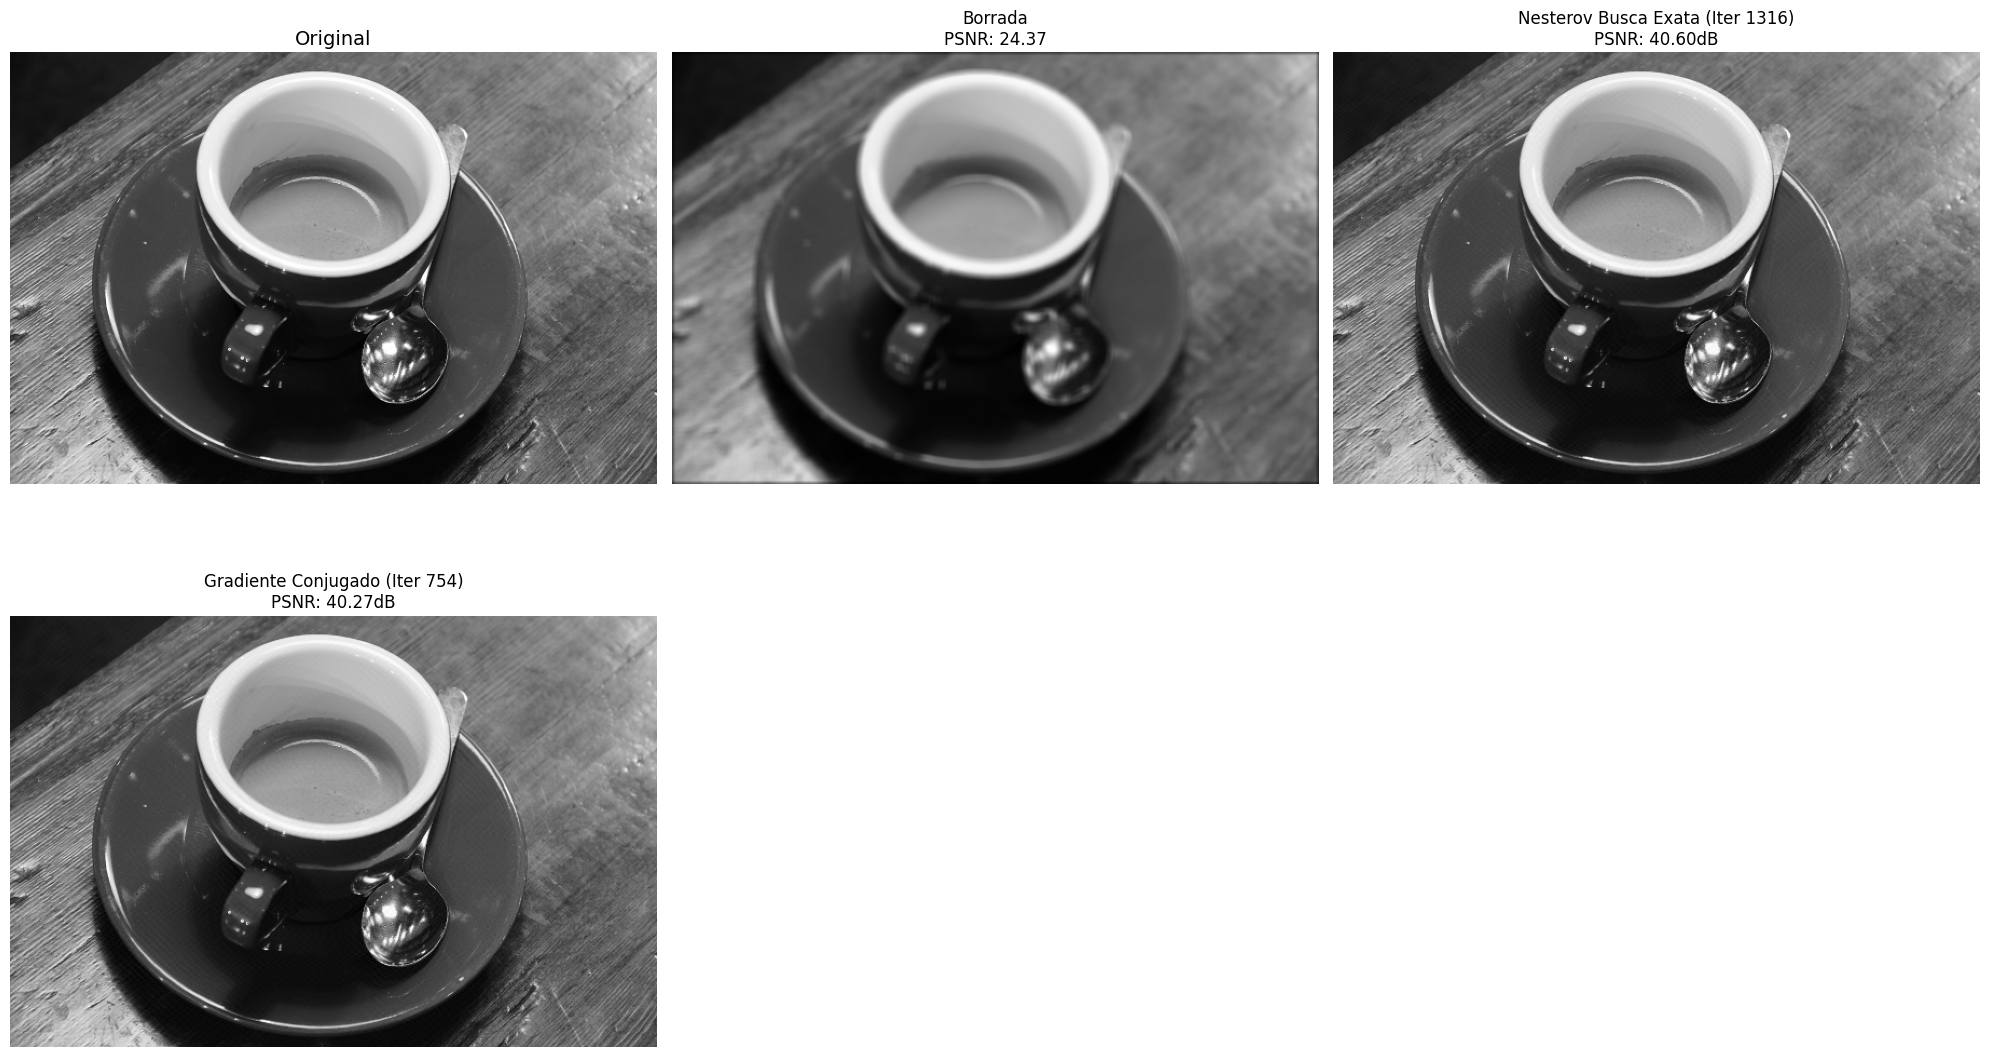
\includegraphics[width = 1\textwidth]{reconstrucao_nest_gc.png}
    \caption{Qualidade da Reconstrução}
    \label{fig:reconstrucao_nest_gc}
\end{figure}

\subsection{Métodos com Regularização para Reconstrução de Imagens}

Em um primeiro momento, consideramos o problema compósito: 

\[
\min F(x) = \frac{1}{2}\norm{Ax - b}_2^2 + \gamma \norm{Hx}_1
\]

onde $A$ é um operador de convolução, $x$ é a imagem a ser recuperada, $b$ é a imagem borrada e ruidosa e $H$ é uma transformada \textit{wavelet}. Para a geração de $b$, foi utilizada a imagem \textit{astronaut} da biblioteca \textit{scikit-image} e foram utilizados um operador de convolução com um kernel de média de dimensões $7 \times 7$ e um ruído gaussiano com média $\mu = 0$ e desvio padrão $\sigma = 0.01$. Para o termo de regularização foi utilizada a \textit{wavelet} de Daubechies. Além disso, foi possível estimar a constante de Lipschitz $L_f = 0.9997$, permitindo assim garantir o limite de convergência teórico para o ISTA ($\lambda < \frac{2}{L_f} = 2.0006$) e para o FISTA ($\lambda \leq \frac{1}{L_f} = 1.0003$). Portanto, o tamanho de passo $\lambda = 1$ foi utilizado para os algoritmos de passo fixo e \textit{backtracking}. Nesta seção utilizamos a norma $\norm{x_k - x_{k-1}}_F$ como critério de parada.

O parâmetro de regularização $\gamma$ foi determinado de maneira empírica, através de um grid search que seleciona o valor que minimiza o erro quadrático em relação a imagem original. Os testes feitos podem ser observados na Figura \ref{fig:params_reg}

\begin{figure}[H]
    \centering
    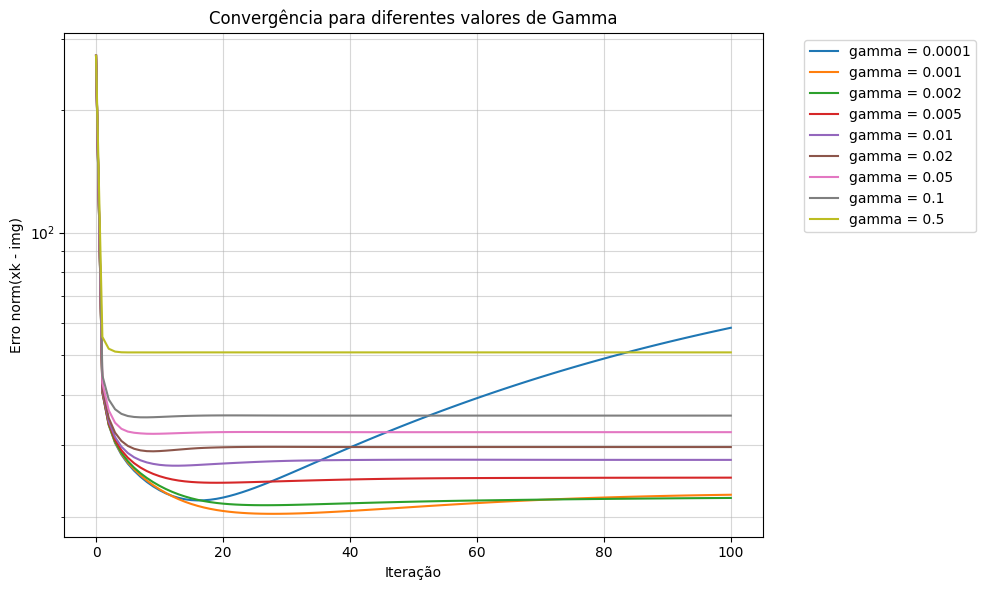
\includegraphics[width = 1\textwidth]{reg_params.png}
    \caption{Análise do erro para diferentes valores do parâmetro de regularização $\gamma$.}
    \label{fig:params_reg}
\end{figure}

Dessa maneira, em um primeiro experimento optou-se pela utilização de $\gamma = 0.001$, um limite de 250 iterações e uma tolerância de $ 1.0 \times 10^{-2}$. Os resultados podem ser observados nas Figuras \ref{fig:f_fstar1} e \ref{fig:fk1_fk}. 


\begin{figure}[H]
    \centering
    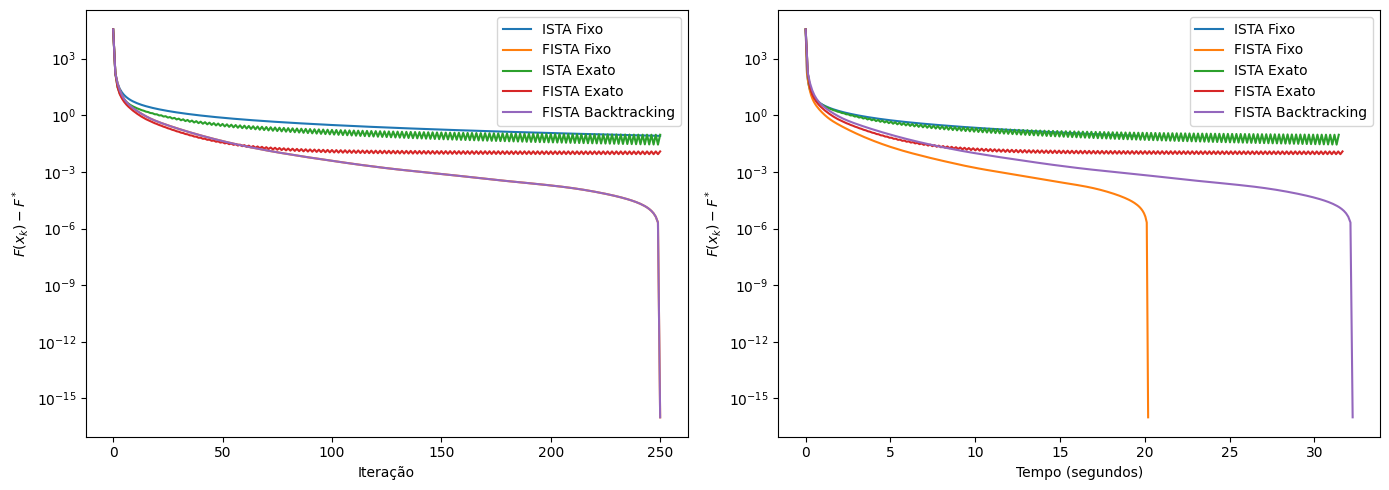
\includegraphics[width = 1\textwidth]{f_fstar1.png}
    \caption{Gráfico da diferença entre $F(x_k) - F(x^*)$}
    \label{fig:f_fstar1}
\vspace{0.2cm}
{\footnotesize Curvas que atingem valores reduzidos em menos iterações e menor tempo indicam melhor desempenho do método. O valor $F(x^*)$ foi definido como o valor mínimo numérico entre todos os algoritmos}


\end{figure}

\begin{figure}[H]
    \centering
    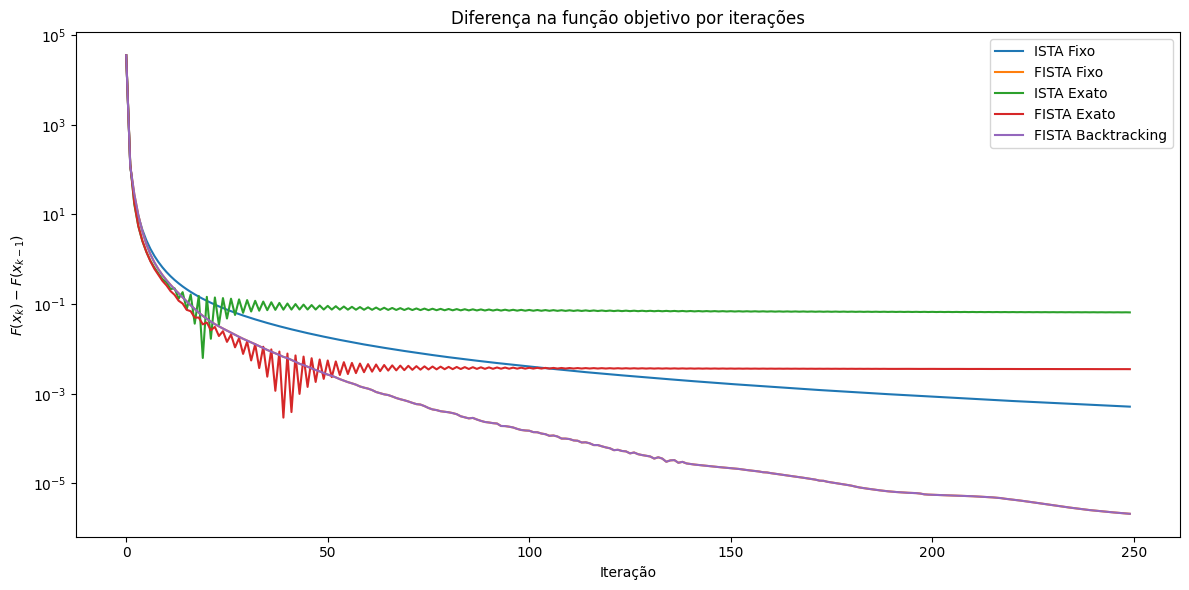
\includegraphics[width = 1\textwidth]{fk1_fk.png}
    \caption{Gráfico da diferença entre $F(x_k) - F(x_{k-1})$}
    \label{fig:fk1_fk}
\vspace{0.2cm}
{\footnotesize Decaimentos estáveis indicam maior estabilidade e que o algoritmo está convergindo de forma consistente para o mínimo. Note que o FISTA Backtracking está sobreposto ao FISTA Fixo.}
\end{figure}

A análise das imagens nos revela que o uso da busca exata, tanto no ISTA quanto no FISTA, compromete a convergência e a estabilidade dos algoritmos. Enquanto as implementações que utilizam passo fixo ou \textit{backtracking} respeitam os critérios de convergência, a busca exata, por ser calculada com base apenas no termo quadrático, negligencia o termo não diferenciável. Isso resulta em passos que não satisfazem a condição de descida para a função compósita, gerando a instabilidade observada. 

Para investigar tal comportamento, podemos ver na Figura \ref{fig:tamanho_passo_creg} que os tamanhos de passo gerados pelos algoritmos não respeitam o limite teórico de convergência, impedindo que os métodos alcancem o mínimo.

\begin{figure}[H]
    \centering
    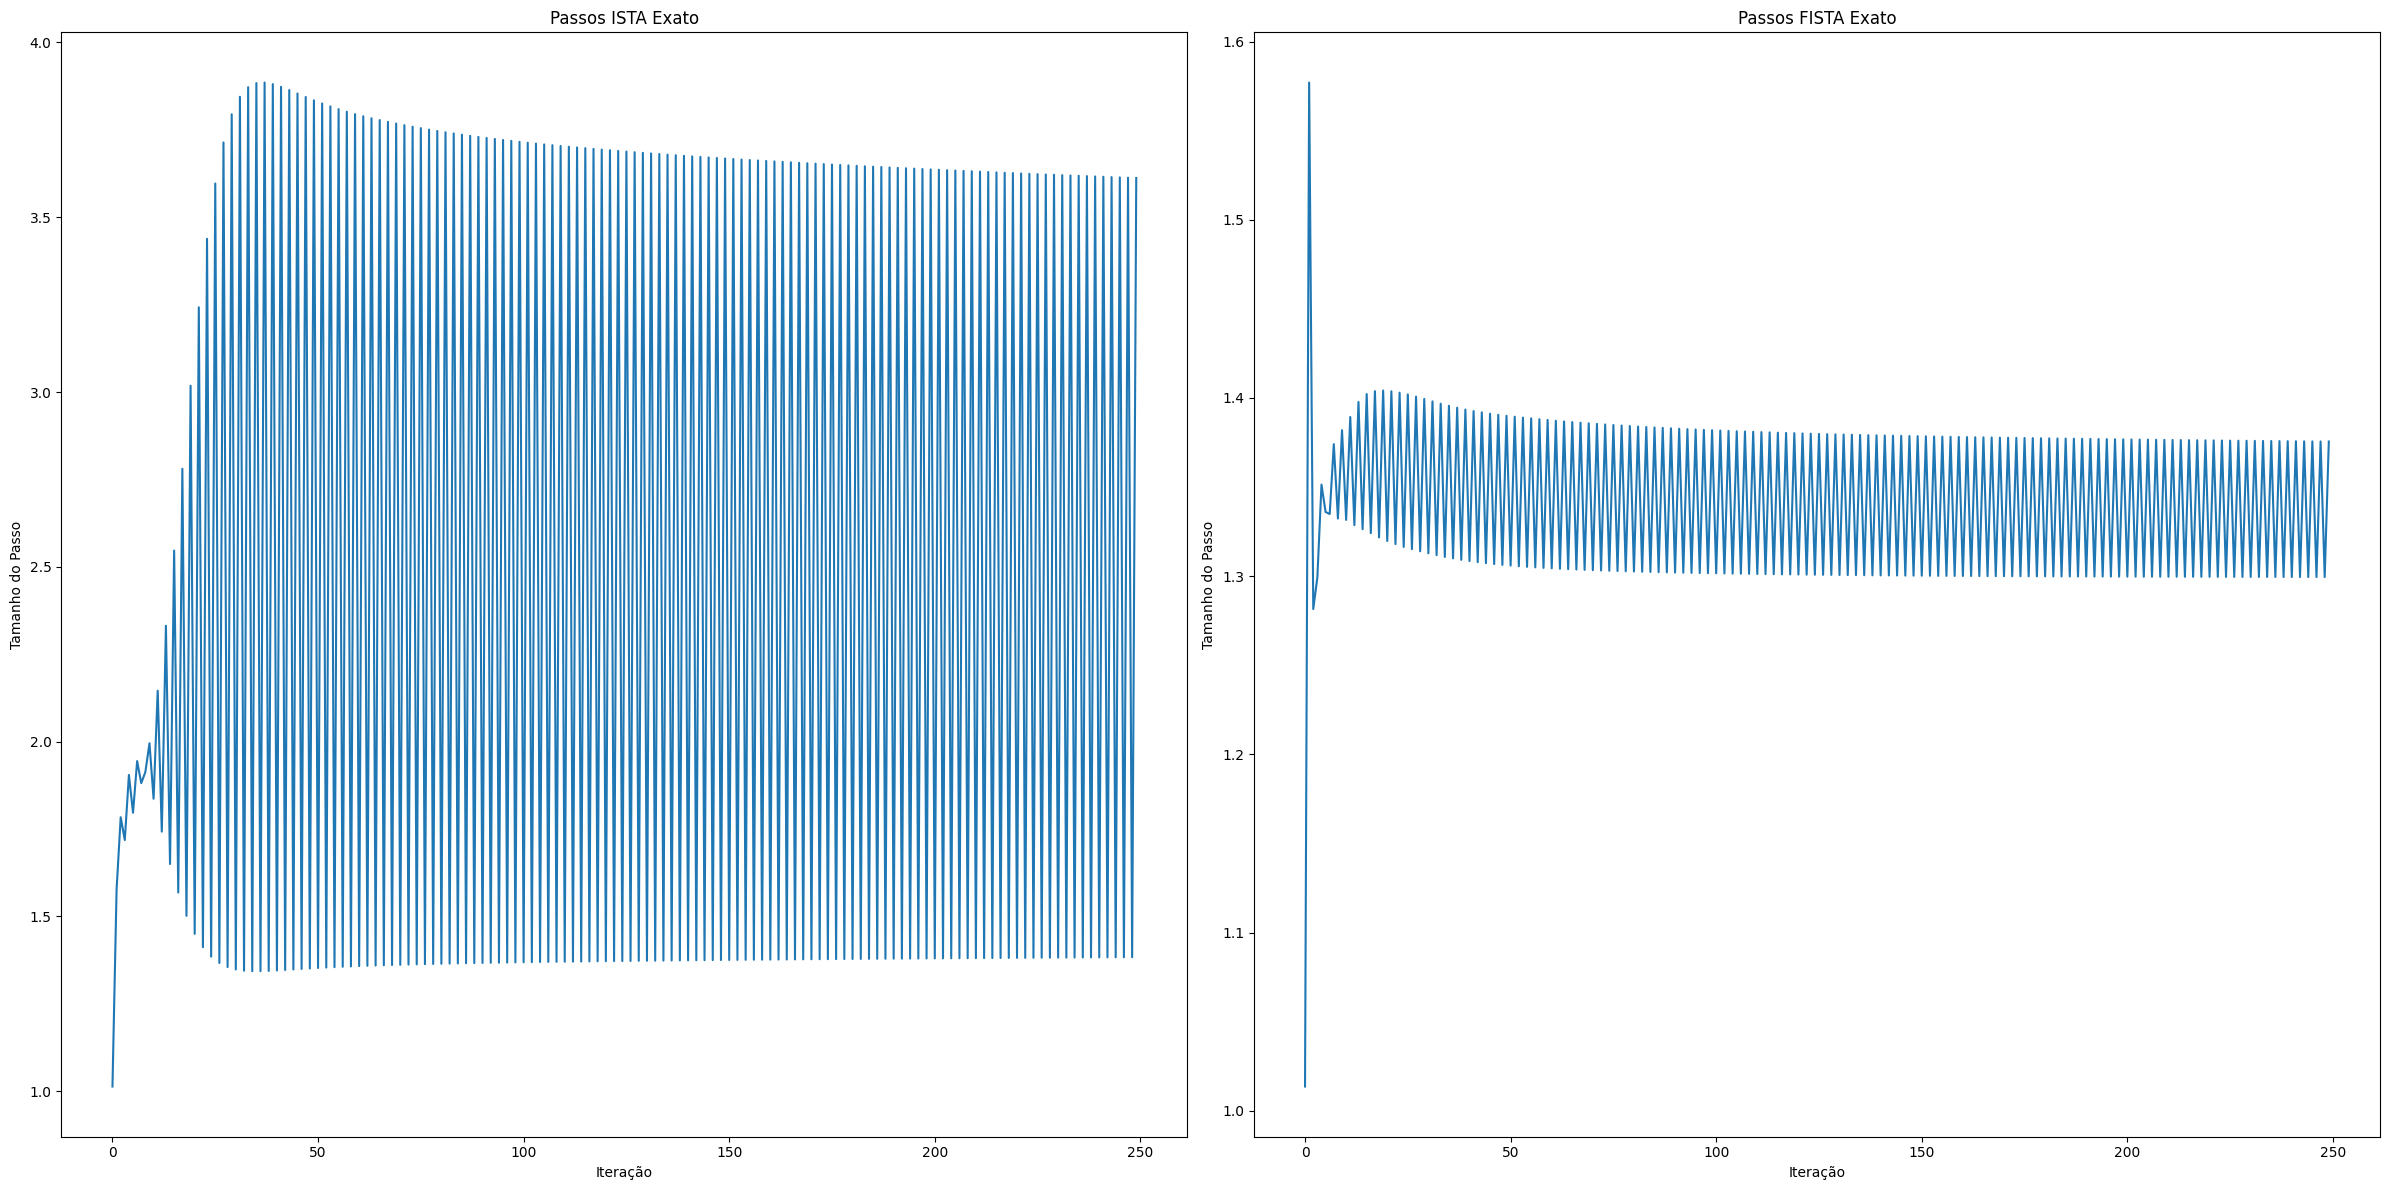
\includegraphics[width = 1\textwidth]{tamanho_passo_creg.png}
    \caption{Tamanho de passo}
    \label{fig:tamanho_passo_creg}
\vspace{0.2cm}
{\footnotesize Note a instabilidade e a quebra do limite teórico de convergência.}
\end{figure}

Para investigar a sensibilidade dos métodos ao termo de regularização, realizaram-se testes com diferentes valores de $\gamma$ (em específico os valores foram $\gamma \in \{0.0001, 0.001, 0.01, 0.1, 0.2\}$), limite de 250 iterações e uma tolerância de $1.0 \times 10^{-2}$. Esses testes justificam-se pelo fato de o passo exato ser calculado com base apenas na parcela suave da função a ser minimizada, tornando-se teoricamente mais adequado ao problema conforme a importância do termo não suave diminui. Os resultados podem ser observados nas Figuras \ref{fig:testes1} e \ref{fig:testes2}.

\begin{figure}[H]
    \centering
    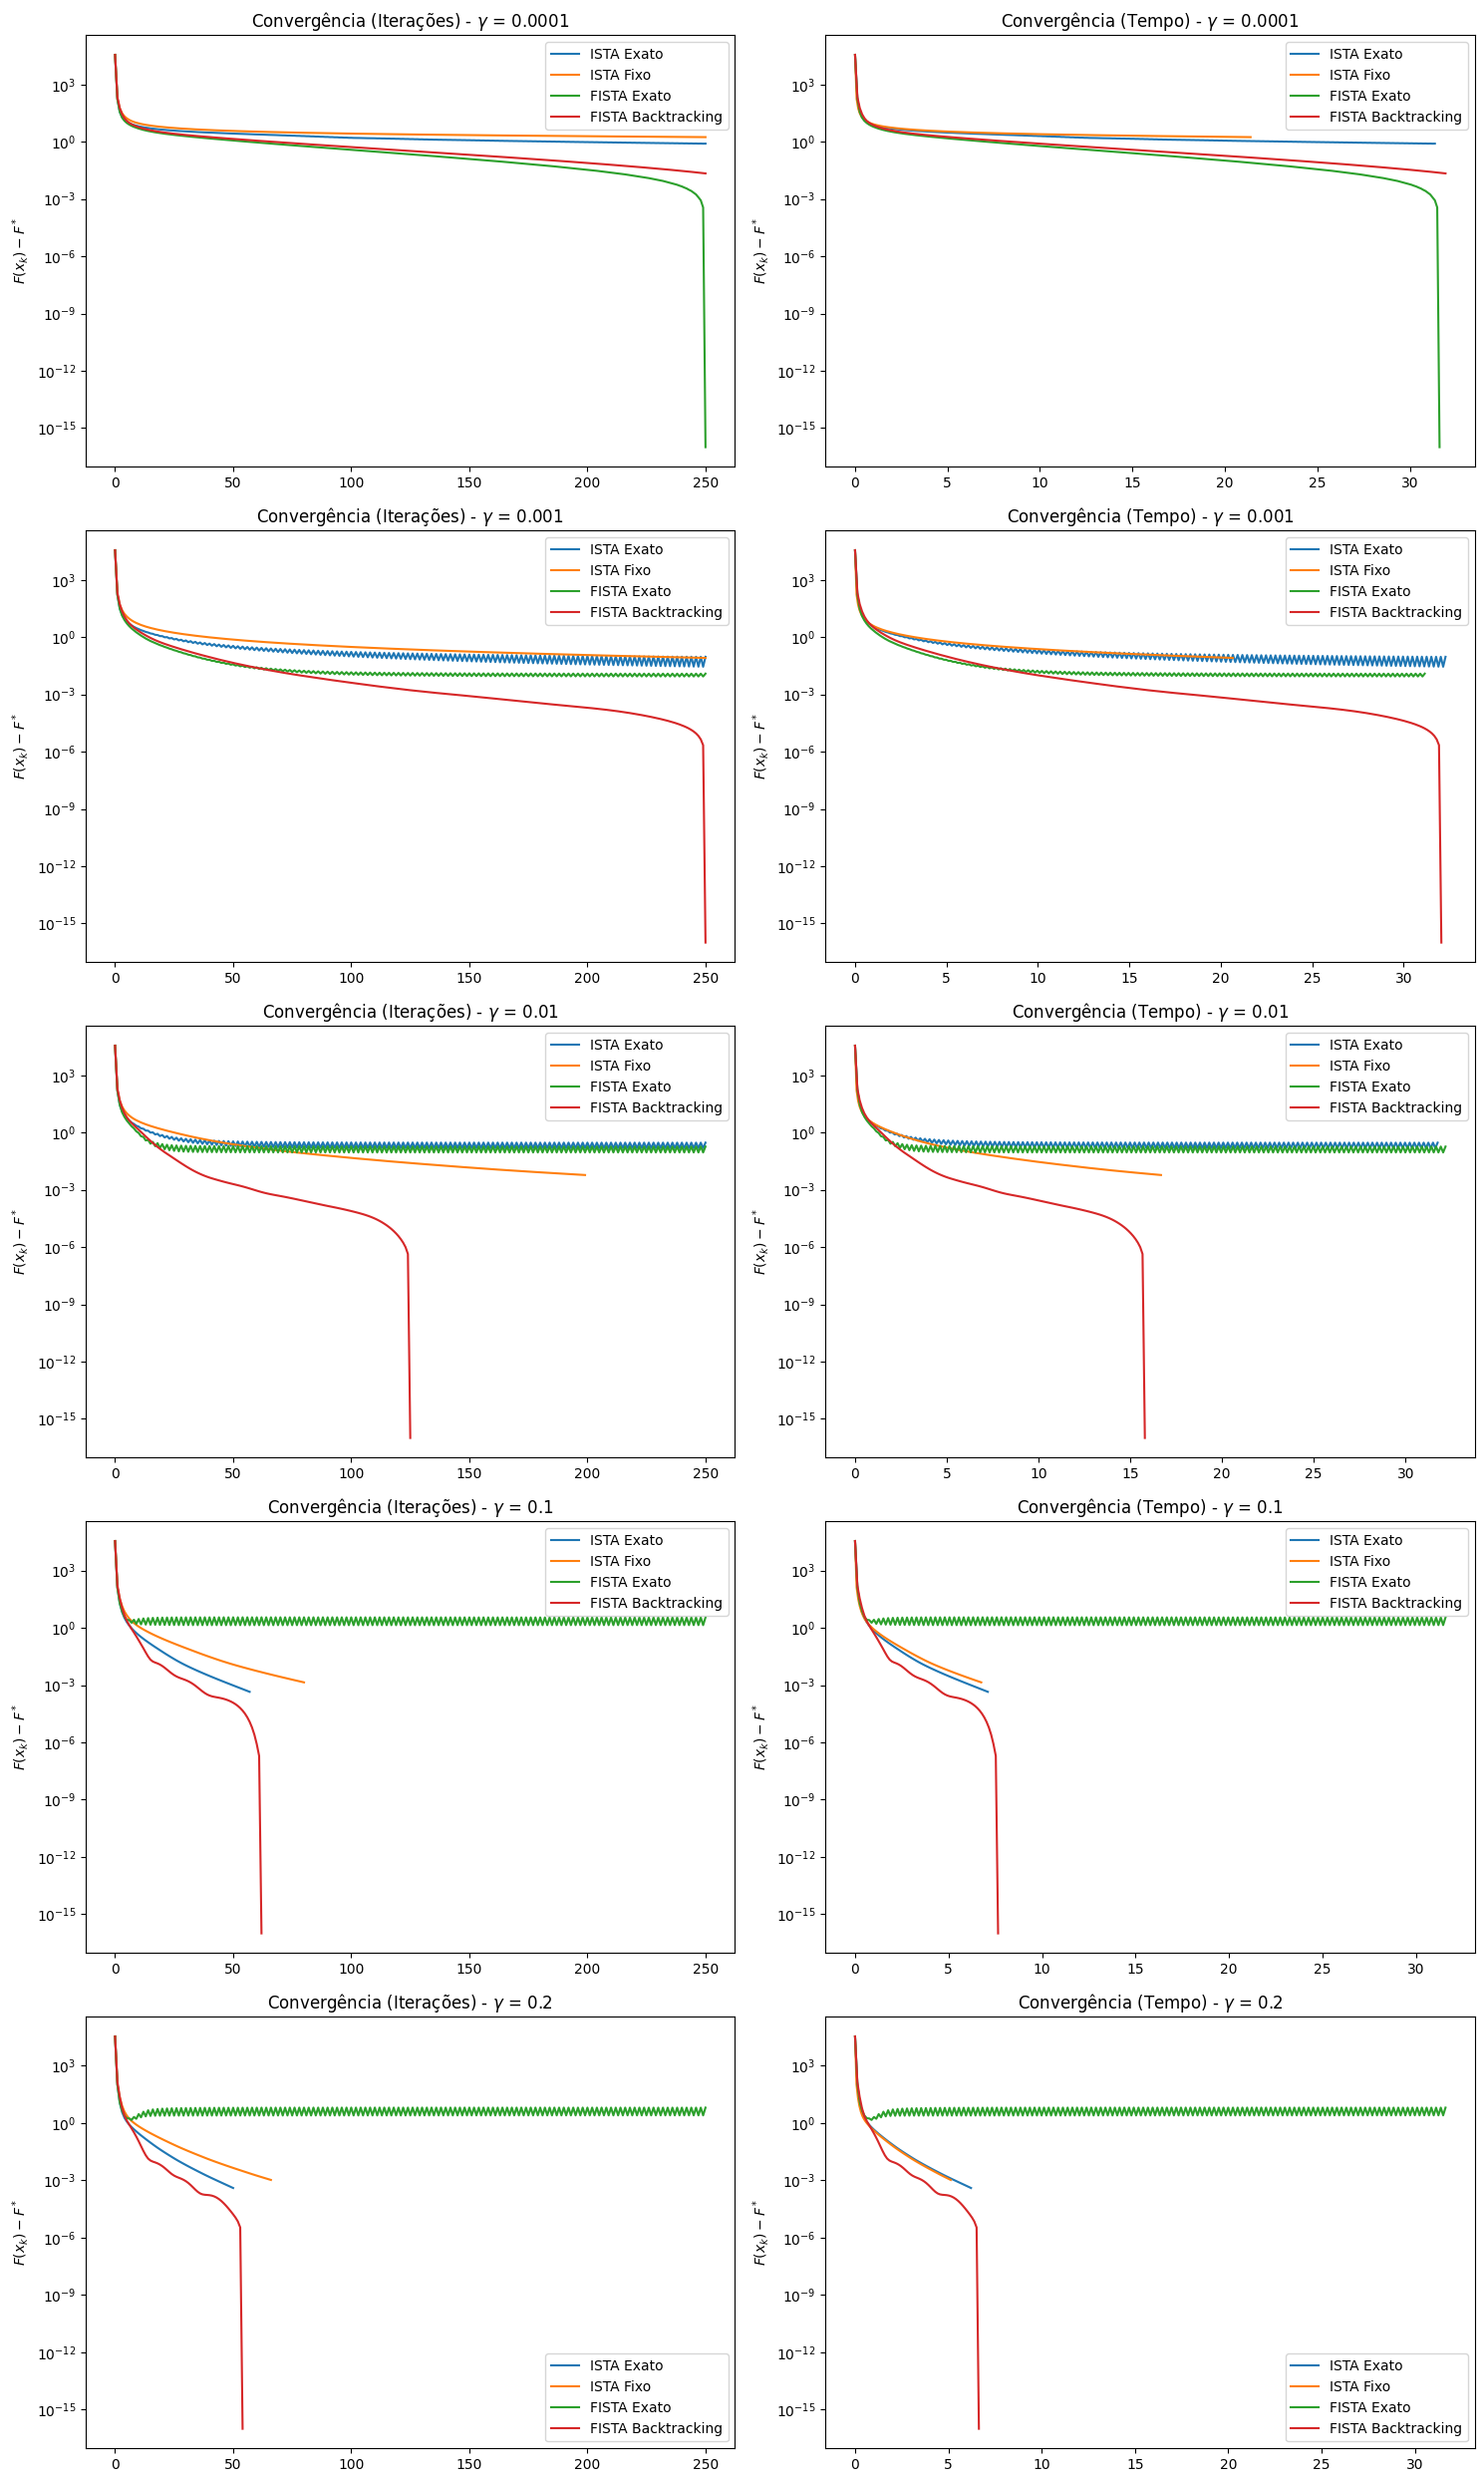
\includegraphics[width = 0.8\textwidth]{testes1_creg.png}
    \caption{Gráficos comparativos de $F(x_k) - F(x^*)$ para diferentes valores de $\gamma$}
    \label{fig:testes1}
\end{figure}

\begin{figure}[H]
    \centering
    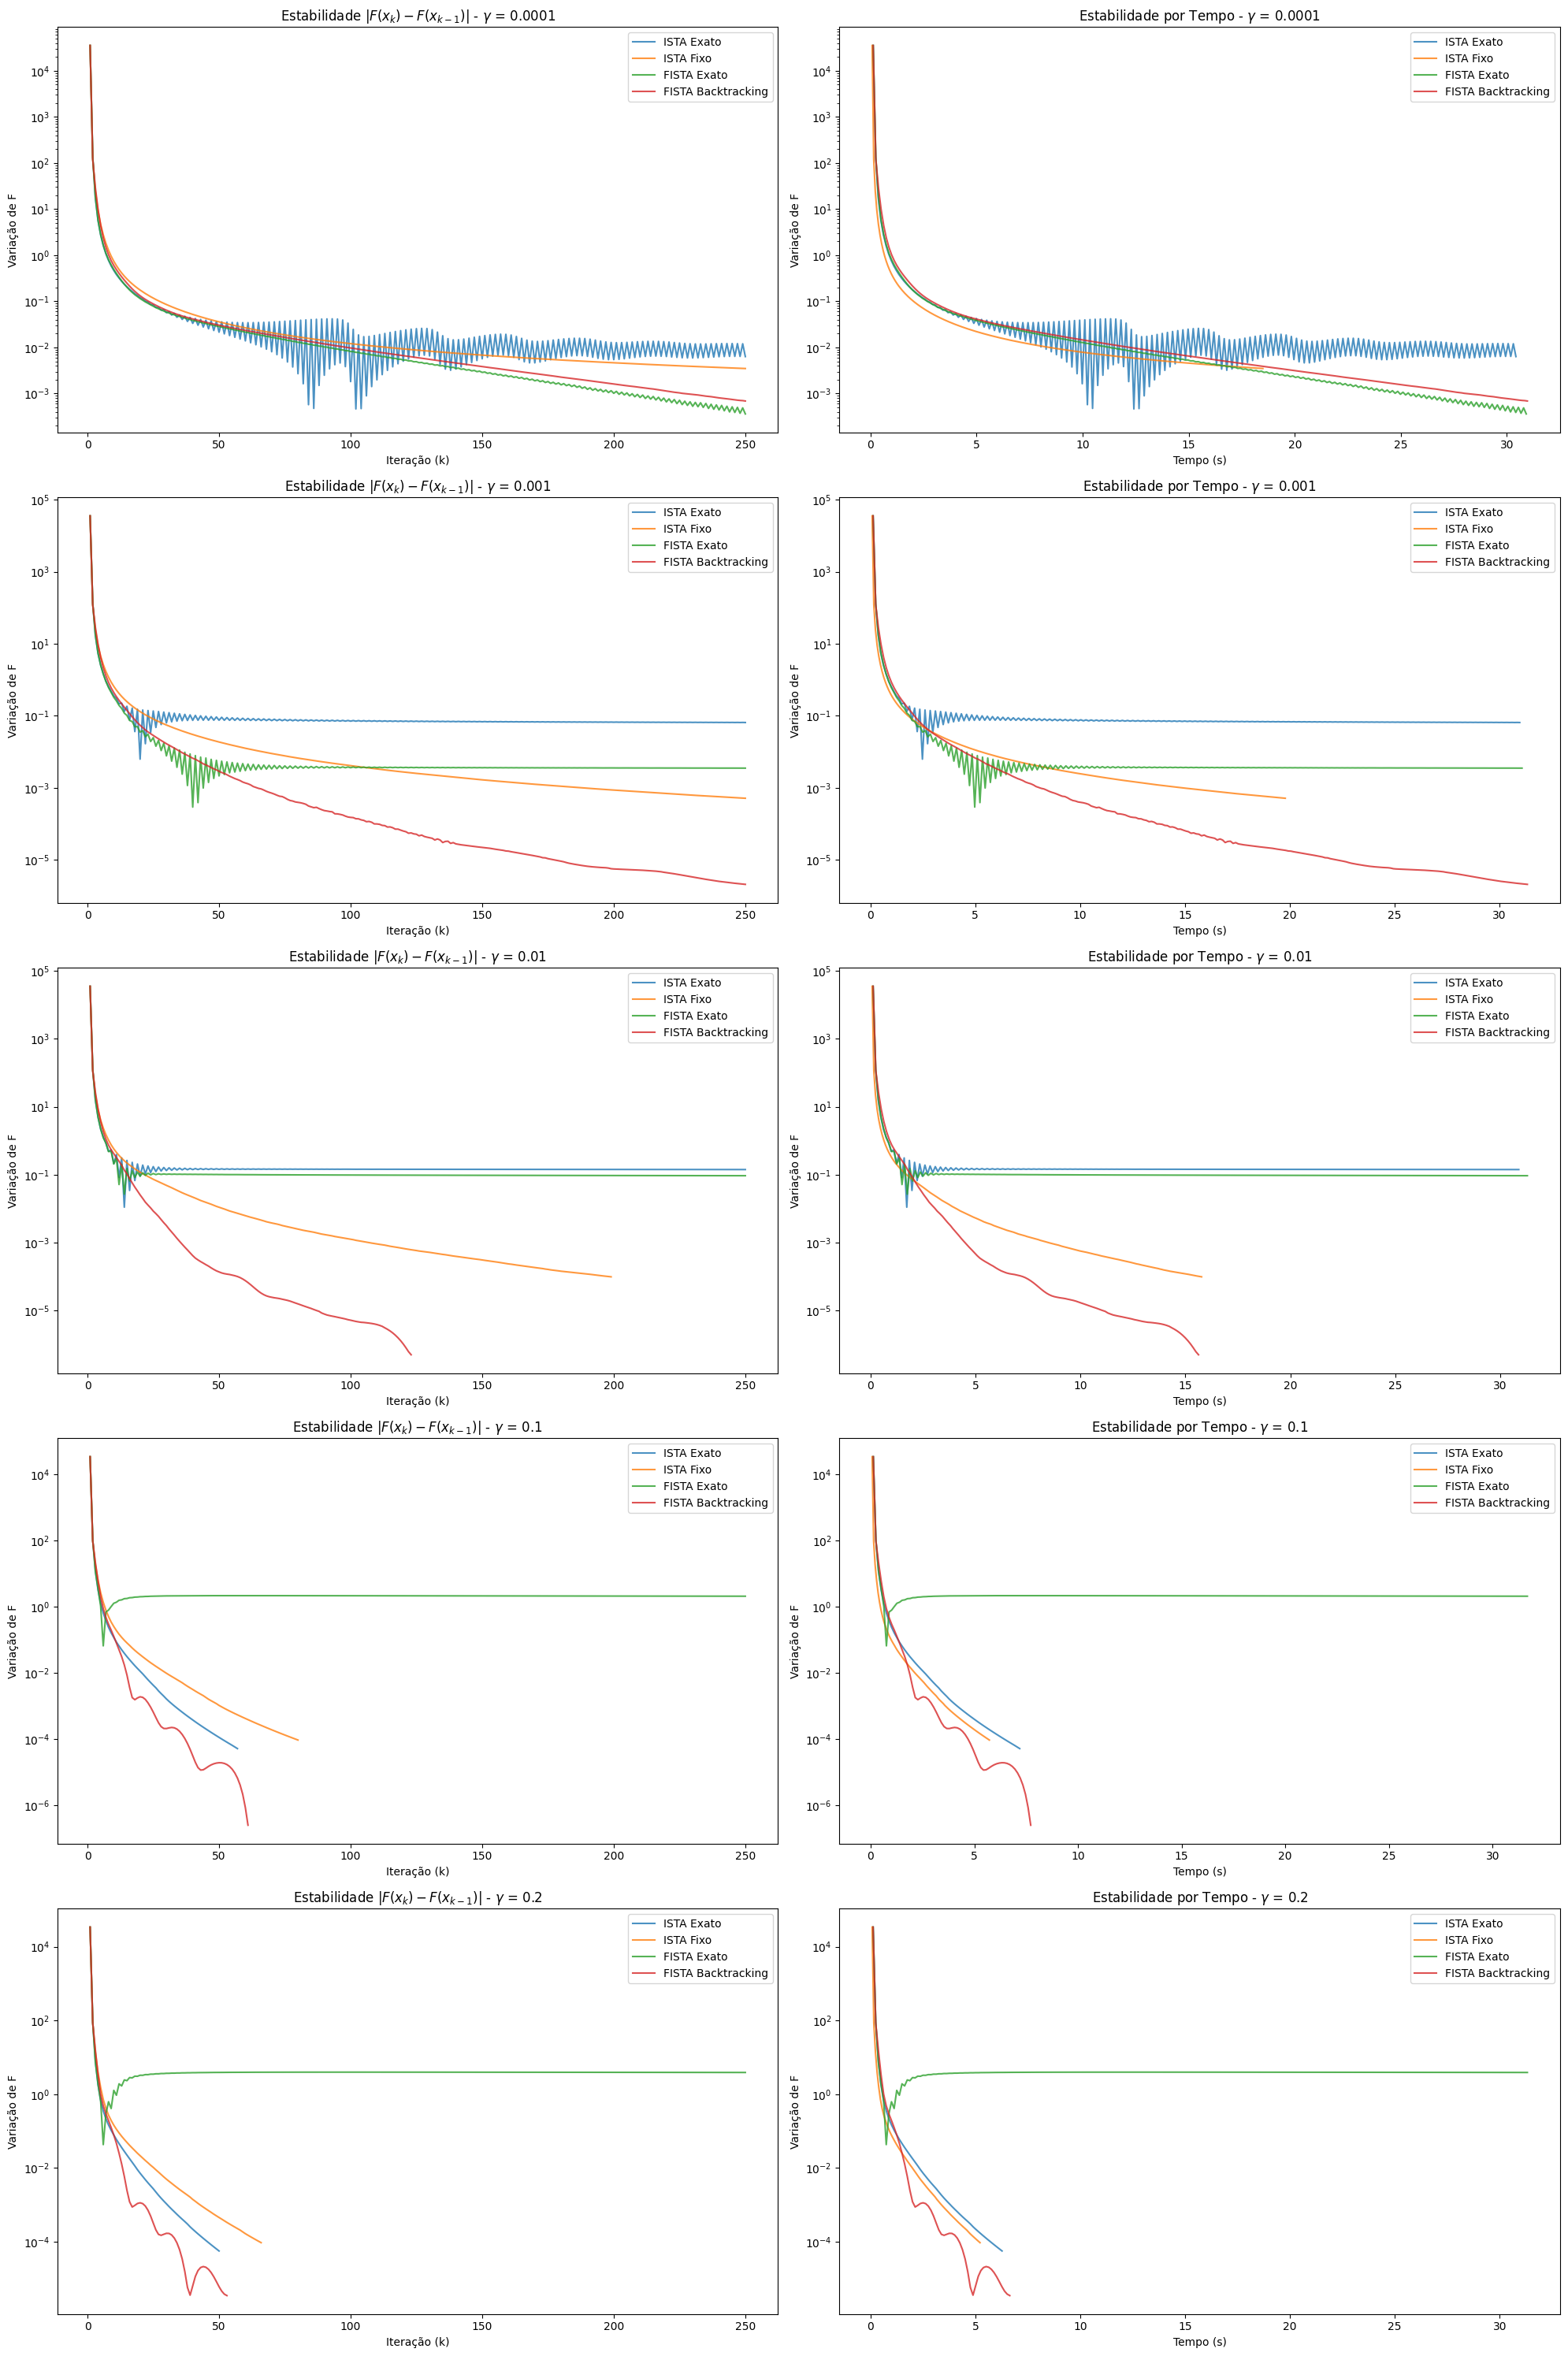
\includegraphics[width = 0.8\textwidth]{testes2_creg.png}
    \caption{Gráficos comparativos de $F(x_k) - F(x_{k-1})$ para diferentes valores de $\gamma$}
    \label{fig:testes2}
\end{figure}

Na Tabela \ref{tab:dif_gammas} pode ser visto um resumo do comportamento dos métodos com passo exato para os diferentes valores de $\gamma$.


\begin{table}[H]
    \centering
    \caption{Comparação para diferentes valores de $\gamma$}
    \label{tab:dif_gammas}
    \begin{tabular}{lcc}
        \toprule
        \textbf{Gamma} & \textbf{FISTA Exato} & \textbf{ISTA Exato} \\
        \midrule
        $0.0001$ & Convergência com oscilações & Convergência lenta e oscilatória\\
        $0.001; 0.01$ & Oscilações sem convergência & Oscilações sem convergência \\
        $\geq 0.1$ & Oscilações sem convergência & Convergência estável\\
        \bottomrule
    \end{tabular}
\end{table}

Veja que para grandes valores de $\gamma$, o operador de \textit{soft-thresholding} impõe uma forte esparsidade à solução. No caso do ISTA, esse efeito favorece a estabilidade do método pois, visto que cada iteração $x_k$ depende exclusivamente de $x_{k-1}$, qualquer passo excessivo é zerado pelo operador de \textit{soft thresholding} e descartado na iteração seguinte. Isso é evidenciado na Figura \ref{fig:norm_diff}, onde a curva azul apresenta um decaimento exponencial da norma $\norm{x_k - x_{k-1}}_F$. Esse comportamento está vinculado à estabilização do tamanho do passo, vista na Figura \ref{fig:passos_gamma_grande}, que permite que o algoritmo convirja para o ótimo. Já no FISTA, a instabilidade persiste. O termo de \textit{momentum} utiliza o histórico das iterações $\beta_k(x_k - x_{k-1})$ para o passo futuro. A consequência disso é que se a busca exata gera um passo grande demais em $x_k$, o erro persiste e é reverberado para $x_{k+1}$, criando um ciclo de oscilações que o operador de \textit{soft thresholding} não consegue suprimir. Esse comportamento pode ser visto nas Figuras \ref{fig:norm_diff} e \ref{fig:passos_gamma_grande}.

Para pequenos valores de $\gamma$ (quando $\gamma \to 0$), temos que a função objetivo se aproxima do problema puramente quadrático, onde vimos na seção anterior que os algoritmos funcionam bem nesse caso.

\begin{figure}[H]
    \centering
    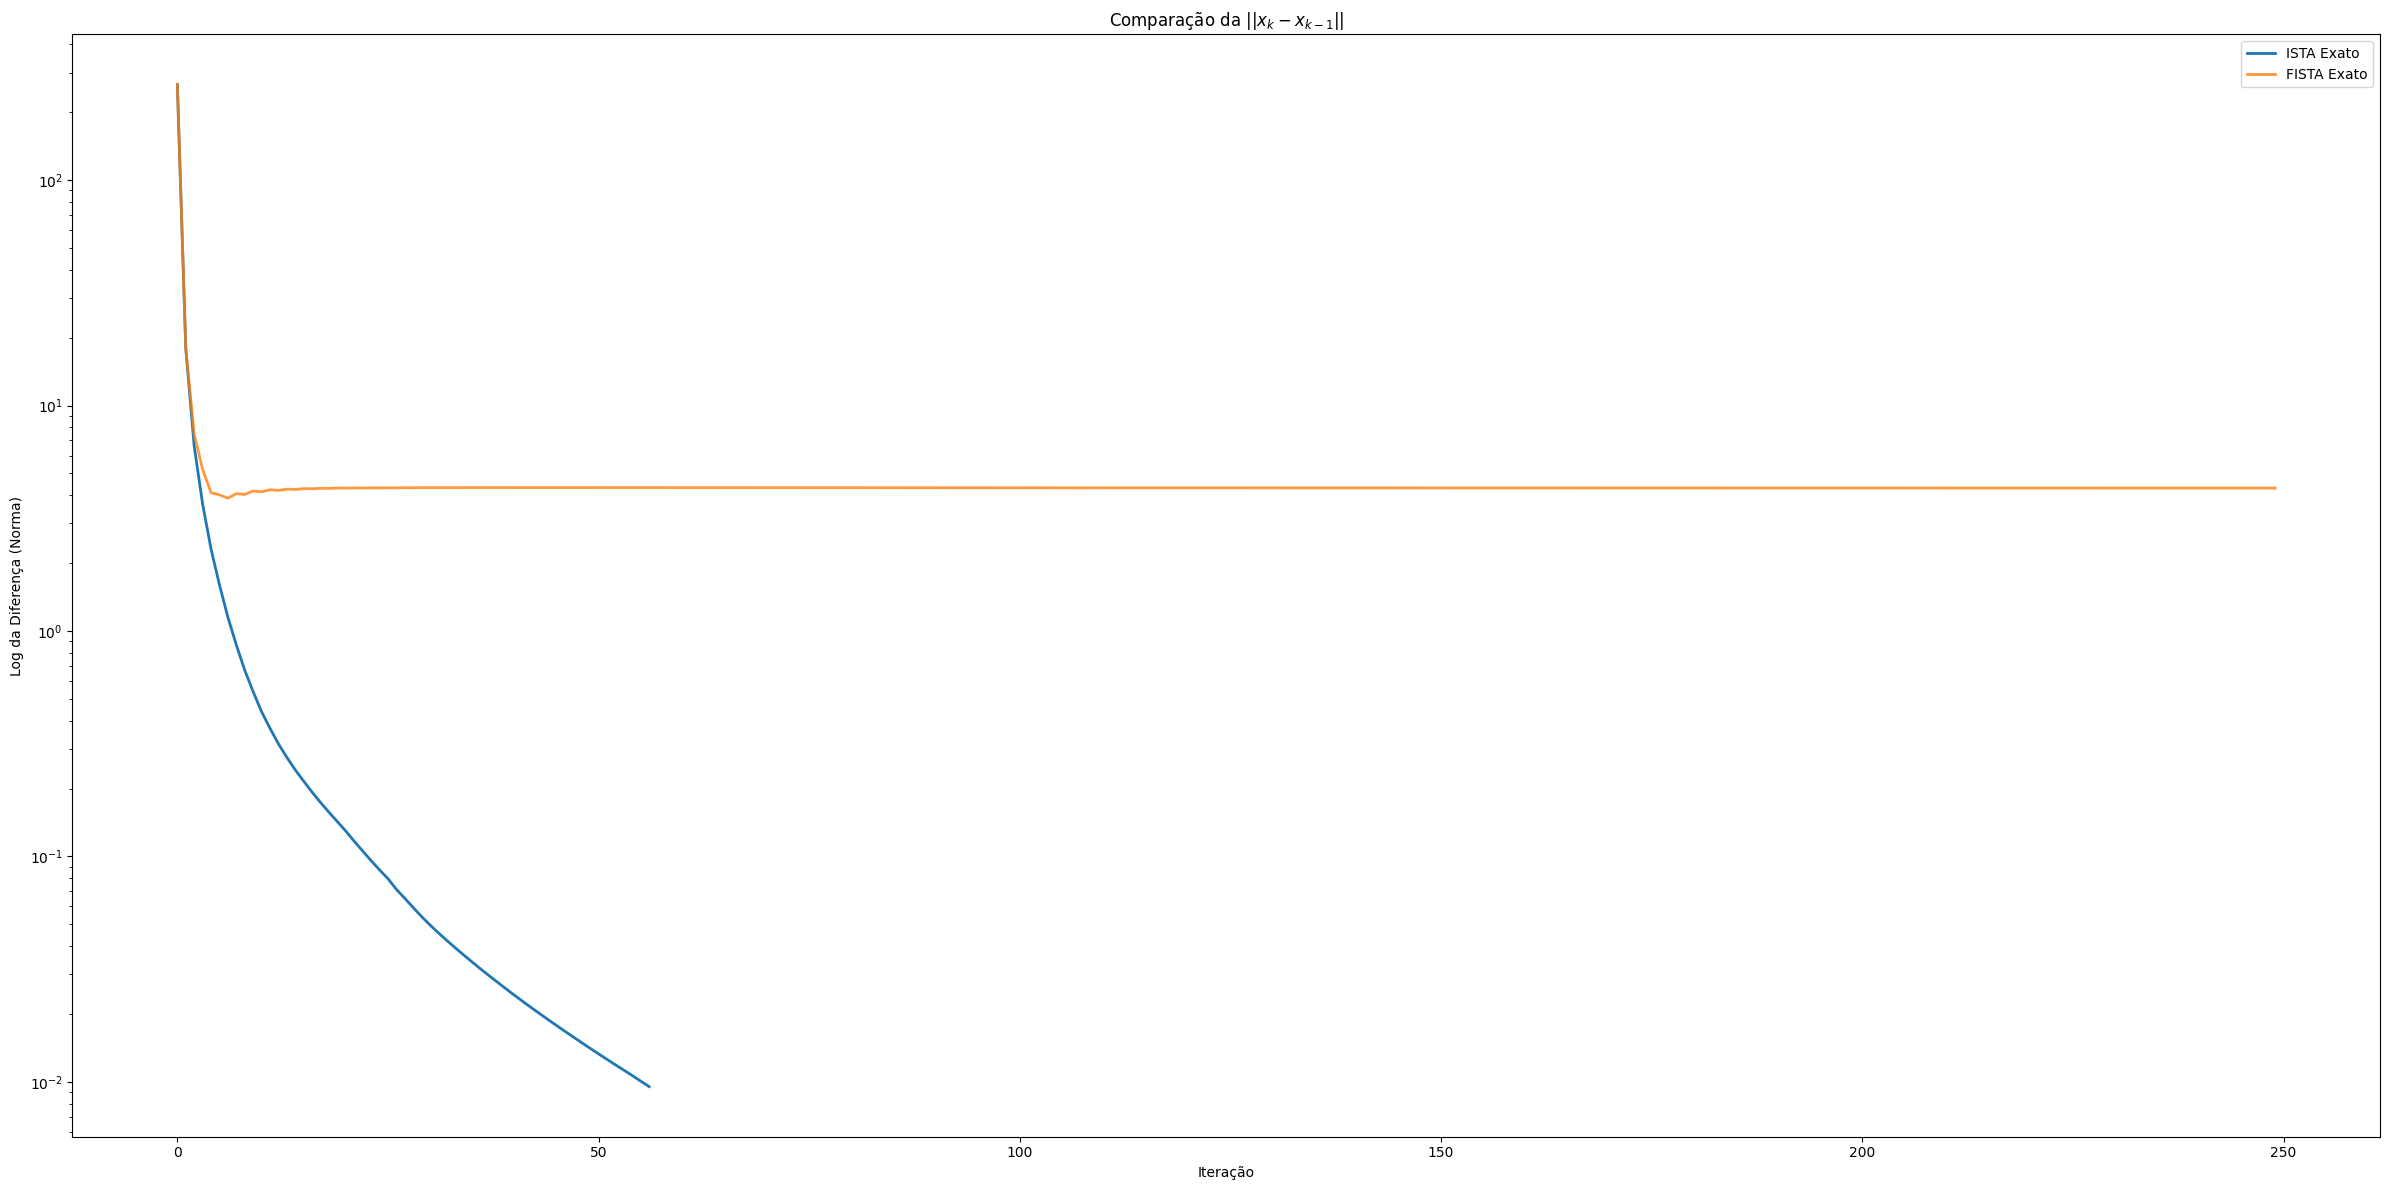
\includegraphics[width = 0.9\textwidth]{norm_xk1_xk.png}
    \caption{Gráfico da diferença $\norm{x_k - x_{k-1}}_F$ para $\gamma = 0.1$}
    \label{fig:norm_diff}
\end{figure}

\begin{figure}[H]
    \centering
    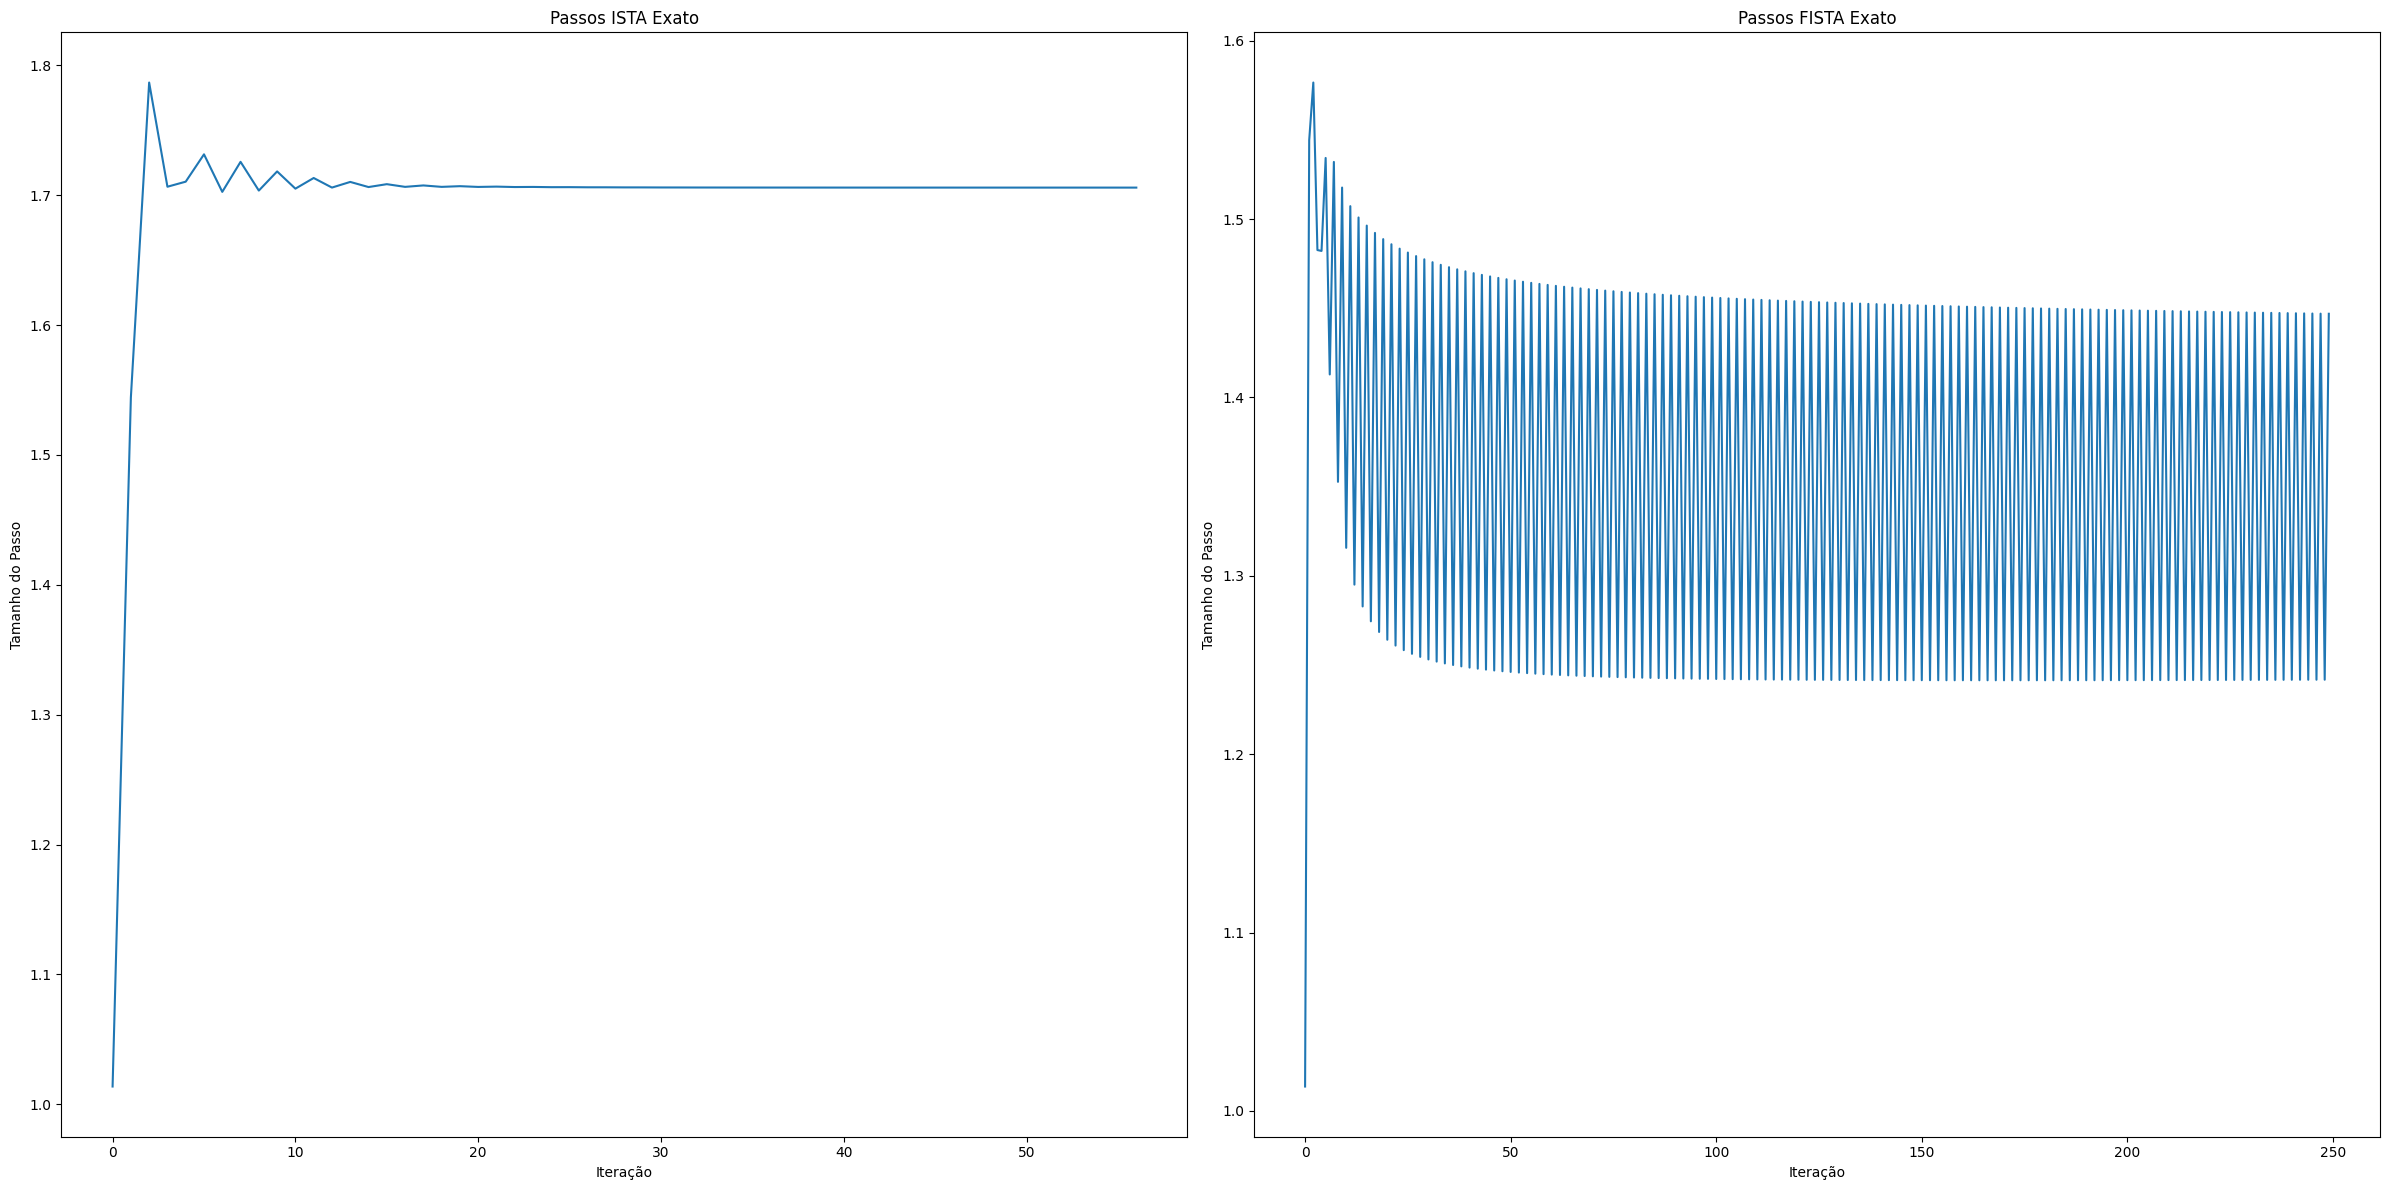
\includegraphics[width = 0.9\textwidth]{passos_gamma_grande.png}
    \caption{Tamanho de passo para $\gamma = 0.1$}
    \label{fig:passos_gamma_grande}
\end{figure}

% \appendix

% \section{Apêndice A: Tamanho de passo máxima descida}
% \label{sec:tamanho_passo}

% O método de máxima descida e o método de Nesterov convergem ao utilizar busca linear exata pelo fato de que para funções suaves a seguinte desigualdade é verdadeira:
% \begin{center}
% $f(y) \leq f(x) + \nabla f(x)^T(y-x) + \frac{L}{2} \norm{y-x}^2_2$    
% \end{center}
% onde L é a constante de Lipschitz.

% Com algumas manipulações que podem ser vistas no Apêndice \ref{sec:tamanho_passo}, chegamos que para o método de máxima descida o algoritmo converge para qualquer tamanho de passo $\lambda < \frac{2}{L}$. Além disso, tomando o tamanho de passo $\lambda = \frac{1}{L}$ obtem-se:

% \begin{center}
%     $f(x_{k+1}) \leq f(x_{k}) - \frac{1}{2L} \norm{\nabla f(x_k)}_2^2$
% \end{center}

% Sendo assim, quando realizamos uma busca linear exata, isto é:
% \begin{center}
%     $\lambda_k = \arg\min_{\lambda \geq 0} f(x_k - \lambda \nabla f(x_k))$
% \end{center}

% Temos que $f(x_k - \lambda_k \nabla f(x_k)) \leq f(x_k - \lambda \nabla f(x_k))$, para todo $\lambda$. Então em particular isso é verdade para $\lambda = \frac{1}{L    }$

% Mas então temos que, de fato:
% \begin{center}
%     $f(x_k - \lambda_k \nabla f(x_k)) \leq f(x_{k}) - \frac{1}{2L} \norm{\nabla f(x_k)}_2^2$
% \end{center}

% e portanto é um algoritmo de descida onde sua convergência é garantida, para checar a demonstração da taxa de convergência basta ver o Apêndice \ref{sec:md_conv}.\\

% No caso do método de Nesterov, a atualização é definida a partir de uma combinação linear das iterações anteriores, gerando um ponto de extrapolação $y_k$. Ao aplicarmos a busca linear exata na direção do gradiente calculado em $y_k$, definimos o tamanho de passo como:

% \begin{equation}
%     \lambda_k = \arg\min_{\lambda \geq 0} f(x_{k+1}) = \arg\min_{\lambda \geq 0} f(y_k - \lambda \nabla f(y_k))
% \end{equation}

% Como $f$ é suave, temos que para um passo fixo teórico $\hat{\lambda} = \frac{1}{L}$, a seguinte desigualdade é válida:

% \begin{equation}
%     f(y_k - \frac{1}{L} \nabla f(y_k)) \leq f(y_k) - \frac{1}{2L} \norm{\nabla f(y_k)}_2^2
% \end{equation}

% Como $\lambda_k$ é o minimizador global da função $f$ ao longo da semirreta $y_k - \lambda \nabla f(y_k)$, segue por definição que o valor da função no ponto obtido pela busca linear não pode ser superior ao valor obtido com o passo fixo $\frac{1}{L}$:

% \begin{equation}
%     f(x_{k+1}) = f(y_k - \lambda_k \nabla f(y_k)) \leq f(y_k - \frac{1}{L} \nabla f(y_k))
% \end{equation}

% Portanto, a busca linear exata herda a garantia de convergência do método original, satisfazendo a condição:

% \begin{equation}
%     f(x_{k+1}) \leq f(y_k) - \frac{1}{2L} \norm{\nabla f(y_k)}_2^2
% \end{equation}

% Embora a convergência seja garantida nesse caso, não há garantias de convergência acelerada.

% \section{Apêndice B: Convergência do método de máxima descida}
% \label{sec:md_conv}

\section{Conclusão}
Neste trabalho, investigamos a influência do uso da busca linear exata para a reconstrução de imagens em algoritmos acelerados de primeira ordem. No cenário de \textit{deblurring} sem regularização, os experimentos demonstram que o método dos gradientes conjugados apresenta o melhor compromisso entre custo computacional e qualidade da reconstrução, superando o método de Nesterov mesmo quando este utiliza a busca linear exata. Observou-se que a busca exata, em comparação ao critério de descida suficiente com \textit{backtracking} reduziu tanto o número de iterações quanto o tempo computacional para o método de Nesterov, embora este ainda se mostre menos eficiente que os gradientes conjugados no caso puramente quadrático. 
Uma etapa subsequente do projeto focará em tentar otimizar a busca exata para o método de Nesterov. Nesse sentido, pretende-se reaproveitar cálculos de produto do tipo $Qd_k$ (ver Proposição 3), visando reduzir o tempo de execução por iteração e tornar o método mais competitivo frente aos gradientes conjugados.

No cenário com regularização $L_1$ (\textit{wavelets}), a busca exata demonstrou-se inadequada. Por ignorar a parcela não suave da função objetivo, o algoritmo frequentemente viola os limites teóricos de convergência, levando a instabilidades. A comparação entre o ISTA e o FISTA revelou que o termo de \textit{momentum} amplifica essa instabilidade. No ISTA, a forte esparsidade promovida ao utilizar $\gamma \geq 0.1$ consegue amortecer as oscilações, fenômeno que não ocorre no FISTA, onde o erro é amplificado ao longo das iterações, impedindo a convergência do método.
As próximas etapas deste trabalho consistem em explorar o uso do passo exato quando o termo regularizador é a variação total (TV) e aplicar esses algoritmos para a reconstrução de imagens de tomografia computadorizada (TC). 


\printbibliography

\end{document}
